\documentclass[12pt]{article}


\usepackage{amsfonts}
\usepackage[parfill]{parskip}
\usepackage{caption}
\usepackage{enumerate} 
\usepackage{booktabs}
\usepackage[pdftex]{graphicx}
\usepackage[top=2cm, bottom=2cm, left=2cm, right=2cm]
{geometry}
%\usepackage[rightcaption]{sidecap}
\usepackage{subfig}
\usepackage [english]{babel}
\usepackage{natbib}
\usepackage [autostyle, english = american]{csquotes}
\usepackage{setspace}
\usepackage[title]{appendix}
%\usepackage[usenames, dvipsnames]{color}
%\MakeOuterQuote{"}
\graphicspath{{./plots/}}
\captionsetup[table]{skip=12pt}
\bibliographystyle{plainnat}







\begin{document}







% ======================================================================================================
% Title page
% ======================================================================================================


\title{The quantification of DNA motifs within flanking sequences of gene expression quantitative trait loci in humans: Laboratory Report}

% Authors
% ----------

\author{Jacqueline Kiewa}





\doublespacing
\maketitle
\clearpage
\tableofcontents
%--------------------------------------------------------------------------------------------------------------------------%
%--------------------------------------- Begin Document -----------------------------------------------------------%


%--------------------------------------------------------------------------------------------------------------------------%
%--------------------------------------- Introduction-------------------------------------------------------------------%
\clearpage
\section{Introduction}

An important complex trait that differs amongst individuals is the level of gene expression, obtained by measuring the amount of mRNA present in specific tissues. The class of variants that influence this trait has been labelled expression quantitative trait loci (eQTL). These variants are particularly important to genome wide association (GWA) studies, since they can help to prioritize likely causal variants amongst the SNPs identified by the GWA study, as well as provide some insight into the biological mechanisms used by organisms to influence complex traits and diseases \citep{albert2015role}. \citet{albert2015role} note that the majority of QTL identified by human GWA studies occur in non-coding regions that are not in linkage disequilibrium (LD) with coding exons. It is therefore hypothesised that these QTL influence their targeted gene through regulation of its expression \citep{nica2013expression}. A further hypothesis is that an eQTL and its surrounding region will be enriched in biologically active DNA elements which will contribute in some way to gene expression regulation. It is argued that the eQTL creates disruption in these DNA elements, resulting in changes in gene regulation. 

\citet{lloyd2017genetic} conducted an analysis using data from the Consortium for the Architecture of Gene Expression (CAGE), which comprises individual-level whole-blood expression and genotype data on 2,765 individuals. This analysis identified a total of 14,995 independent eQTL, of which 11,204  were located proximal to their transcript (i.e., \emph{cis}). In particular, \emph{cis}-eQTL were defined to be those associations such that the SNP was located on the same chromosome as the gene and \emph{trans}-eQTL the complement of this. The aim of this research is to identify DNA motifs in the genomic regions surrounding the set of \emph{cis}-eQTL identified by \citet{lloyd2017genetic}, following the hypothesis that flanking sequences of an eQTL will be enriched in recurring motifs of DNA that have a biological function, most likely involved in transcription.

The overarching hypothesis of this research project is that if DNA motifs are detected in the sequences that surround eQTL then we would expect them to have a common regulatory process across a subset of genes that harbour eQTL in the nearby region. We are searching for a conserved set of mechanisms across blood gene expression that acts through DNA motifs. This project sought to establish first whether it is indeed the case that DNA motifs can be detected in a robust manner using large scale computational techniques applied to a large set of sequences. Secondly, these analyses are intended as a starting point for further investigation into the global role of motifs in  gene expression regulation in regions of the genome that harbour genetic variants that contribute to variation of gene expression in whole blood. 

The report structure is as follows: Section 1 outlines the 
primary hypothesised biological role of motifs in DNA to clarify the potential importance of motifs and their link with eQTLs. Modes of motif detection in vivo, in vitro and in silico are described, and the latter exemplified with a conceptual example of motif detection algorithms. This section also introduces the notation used in this report and some key concepts. Section 2 outlines the purpose and main results of a pilot study, which motivated key choices in study design for the primary study.  Section 3 summarises the study design and resources used for the primary study before providing a detailed description of results. Sections 4 and 5 highlight some of the key conclusions of the study, summarises the primary lessons learnt and the caveats of the study, and then looks to future work. 
 
\subsection{Motif function}
DNA sequence motifs are short, recurring sequences in DNA that are thought to have some biological function \citep{d2006dna}. They may form binding sites for proteins such as transcription factors or nucleases, or they may provide signals for important regulatory processes such as methylation, ribosome binding or mRNA processing \citep{d2006dna}. Gene regulation is an important aspect of the eukaryotic genotype \citep{beckerman2005gene}, changes in which are responsible for much of the phenotypic divergence between and within species \citep{stewart2012transcription}. However, an understanding of the biological mechanisms by which this diversity regulates gene expression has been challenging  \citep{pai2015genetic, gaffney2013global}. Transcription constitutes the first and one of the most intensely regulated steps of gene expression \citep{zabidi2016regulatory}, and a subset of DNA motifs in the region of eQTL are sequence binding sites for transcription factors (TFs). Much research has therefore focused on the identification of transcription factors that coincide with eQTL and are likely to enhance or restrict gene expression. 

Once chromatin has become accessible, transcription can initiate within the core promoter site, which recruits RNA polymerase II and assembles the pre-initiation complex \citep{zabidi2016regulatory}. However, transcription will proceed at a very low basal level without the contribution of enhancers. Enhancers are DNA elements up to several hundred base pairs in length, and contain many short TF binding sites. Either individual or cooperative combinations of TFs are recruited to these sites and function as activators or repressors that regulate transcription from the target core promoter. Despite the abundance of research that has focussed on the relationship between eQTL and transcription factors, as a subset of DNA sequence motifs, TFs form just one piece in the complex jigsaw of gene regulation, with other regulatory processes also playing a part. A de novo motif search by \citet{schor2017promoter}, for example, found a number of core motifs (not TF binding sites) that controlled the shape of promoter regions, resulting in changed transcription levels. Other systems of gene regulation include methylation of CpG sites, alternative splicing, and post-transcriptional effects such as interaction with miRNAs and polyadenylation \citep{gaffney2013global}. \citet{gaffney2013global} also observed that eQTL are often enriched in exons, and \citet{kirsten2015dissecting} found that eQTL also coincide with non-coding RNAs and pseudogenes.
 
The following overview of potentially important motifs in DNA follows that of \citet{boeva2016analysis}. Tandem repeats are a repeated DNA sequence ordered in a head-to-tail fashion and include microsatellites, minisatellites, and satellite sequences. Short tandem repeats (STRs) may serve as binding sites for specific transcription factors, whilst longer satellite repeats can influence the three dimensional structure of the genome. Interspersed repeats are similar sequences to STRs and are located throughout the genome and include transposable elements such as short and long interspersed nuclear elements.. 

AT-rich sequences are often located in gene promoters and play a role in transcription initiation. Approximately 24\% of human genes contain an AT-rich sequence within the core promoter, with 10\% containing a canonical TATA-box motif (TATAWAWR; W = A/T, R = A/G). In general, AT-rich DNA is easier to unwind than GC-rich DNA, since AT base pairing contains fewer bonds than GC base pairs, but this process is amplified by the TATA binding protein which is recruited by the TATA-box. 

The remaining 76\% of human promoters that are GC-rich contain multiple binding sites of the transcriptional activator SP1 \citep{yang2007prevalence}. As much as 56\% of human genes, including most housekeeping genes, possess CpG islands, i.e. 300-3000 base pair GC-rich sequences around gene transcription start sites (TSSs) with a high density of CpG dinucleotides. CpG islands have a high methylation level, which is associated with transcriptional repression. 

Splice sites are involved in post initial transcription, when the RNA undergoes the process of splicing, during which introns are removed and the remaining exons are joined together. Generally this process is catalyzed by spliceosomes that recognize a donor site, which is almost invariably `GU' at the 5' end of the intron; a branch site, which is an `A' followed by a pyrimidine-rich tract near the 3' end of the intron; and an acceptor site, which is almost always `AG' at the 3' end of the intron. A DNA mutation in a splice site may have a wide range of functional consequences often leading to a defective or truncated protein.  

Micro RNA molecules (miRNAs) regulate the amount of protein at the post-transcriptional level. Micro RNAs form part of the RNA-Induced Silencing Complex (RISC). The function of miRNA in this complex is to bind to the 3' untranslated region of of messenger RNA (mRNA). A successful binding will lead to repression of the translation of mRNA into protein. Mutations in an miRNA target site can therefore disrupt miRNA repressive regulation, resulting in protein over expression.

This short summary of biological mechanisms for the regulation of gene or protein expression highlights binding sites, or motifs, as the common factor within each regulatory process. The abundance of potential motif mechanisms has motivated research into tools for detecting their presence within the DNA sequence, with the intent of deciphering the gene regulatory program. 

\subsection{Motif detection}
DNA motif detection can be done experimentally or with high-throughput data analysis using computer algorithms. Identification of DNA motifs can be achieved through in vivo or in vitro experiments, which include, for example, ChIP-seq (in vivo) that uses actual TF binding events in particular biological conditions, such as cell type or treatment time point \citep{inukai2017transcription}. In vitro approaches (e.g. SELEX) use artificially created DNA and are well suited for large-scale characterization of intrinsic TF binding sequence preferences \citep{inukai2017transcription}.  Results from a ChIP-seq experiment typically have a resolution of approximately 100 base pairs, and the set of sequences identified as a result of the experiment (ChIP-seq data) becomes the focus of a search for a single motif for the particular transcription factor used within the binding experiment, i.e. one motif that is the best match over all sequences identified within the experimental process. This process has been termed one occurrence per sequence (OOPS) \citep{zhang2016entropy}. This consensus motif is putatively labelled as a transcription factor binding site (TFBS) for the bound transcription factor identified within the experimental data. 

Alternatively, computational based motif detection searches for short lengths of DNA that are conserved across sequences, but is not limited to one motif per sequence or to TFBSs. Zero, one, or multiple different motifs per sequence (respectively called `ZOOPS', `OOPS' and `MOPS') can be identified. The conservation of these motifs is thought to indicate biological significance. This significance is not necessarily that of a TFBS, but might be due to some other factor, as described in Section 1.1 above. 
Multiple computational motif finding tools were first developed for finding transcription factors \citep{dassi2016dynamit}, and many of them require ChIP-seq sequences as input. Later tools were developed to find other motifs, but again often focused on a particular section of DNA, such as promoters or enhancers  \citep{boeva2016analysis}.

\citet{das2007survey} describe motif discovery as one of the most challenging problems in molecular biology and computer science, and formulate it as follows:
given a set of sequences, find an unknown pattern that occurs frequently. If a pattern of $m$ letters long appears exactly in every sequence, a simple enumeration of all $m$-letter patterns that appear in the sequences gives the solution. To find this pattern, in a set of $t$ sequences of length $n$, we need to consider all $(n - m +1)t$ possible starting positions or candidates for motifs. 

The problem increases in complexity with the introduction of $d$, which is the number of point changes that will be accepted in any motif instance. This change might take the form of a simple change in nucleotide (e.g. from an A to a T) or of an insertion or a deletion. Since an exact match may not exist, the motif detection algorithm must consider all possible combinations of `words' of the given length across all sequences. Thus the problem becomes exponential with the number of sequences. For each combination, the detection algorithm must perform an alignment and calculate the probability that this combination of `words' are instances of the same motif. At the end of this process, the combination of `words' with the best probability will become the basis for a position weight matrix (PWM) \footnote{The position weight matrix will be explained more fully in  Section 1.3} which will be the accepted consensual motif for this group of sequences. 

Given this level of complexity, the motif finding problem is an example of an NP-complete problem \citep{tran2014survey} (NP $=$ nondeterministic polynomial time). A solution to the search problem can theoretically be found and verified in polynomial time (with respect to the size and number of sequences) by a nondeterministic algorithm which has the power of guessing correctly at every step \citep{dasgupta2006algorithms}. However, although such an algorithm theoretically exists, no polynomial time algorithm has yet been discovered for this NP-complete algorithm \citep{cormen2009introduction}.  Algorithms for solving this problem can be categorised as per \citet{sun2015affinity}, who grouped algorithms into exact algorithms, which achieve efficiency through organisational pre-processing such as a suffix tree to reduce the search space; and approximate algorithms, which use heuristic methods in combination with optimisation methods such as expectation-maximisation to reduce processing time.
\newpage
\subsection{Conceptual example of a motif detection algorithm, and the position weight matrix}
This section will be used to describe one motif finding algorithm: the Gibbs algorithm \citep{Lawrence1993Gibbs}. A conceptual example will be provided, following that presented in \citet{jones2004introduction}. The concepts presented in this section underpin many of the algorithms
used in the main data analysis and thus provide an intuitive look into the black box of the algorithms that pervade the computational motif search problem. 

The example begins with a set of  $t=4$ sequences of length $n=10$, in which we are to find one example of a motif $M$ of length $l=7$ in each sequence:
\begin{center}
A  C  C  A  T  G  A  C  A  G\\
G  A  T  T  A  T  A  C  C  T\\
C  A  T  G  C  T  T  A  C  T\\
C  G  G  A  A  T  G  C  A  T\\
\end{center}
The algorithm works through repeated iterations of a single process. Each iteration ends with a choice of starting position for the motif in one of the sequences.

An iteration begins by setting one sequence aside as the target sequence. This sequence is chosen randomly, but in this example, the first sequence (marked in red in Figure \ref{gibbs1}) will be used as the random sequence. All other sequences form the background; the background sequences are used to create a frequency table, which is then used to calculate the probability of the motif occurring at each possible position in the target sequence.

To construct the frequency table, first a motif position is chosen, at random, for each background sequence. In Figure \ref{gibbs1} the background motifs are marked blue. Next the blue elements in the table are filled in according to the counts of the nucleotides for each position in the background motifs. The column headers in the table indicate the positions in the motifs. The green column (with the zero header) is filled in according to the counts of nucleotides in the non-motif background, irrespective of position. Figure \ref{gibbs1} illustrates the process:

\begin{figure}[htbp]
\centering
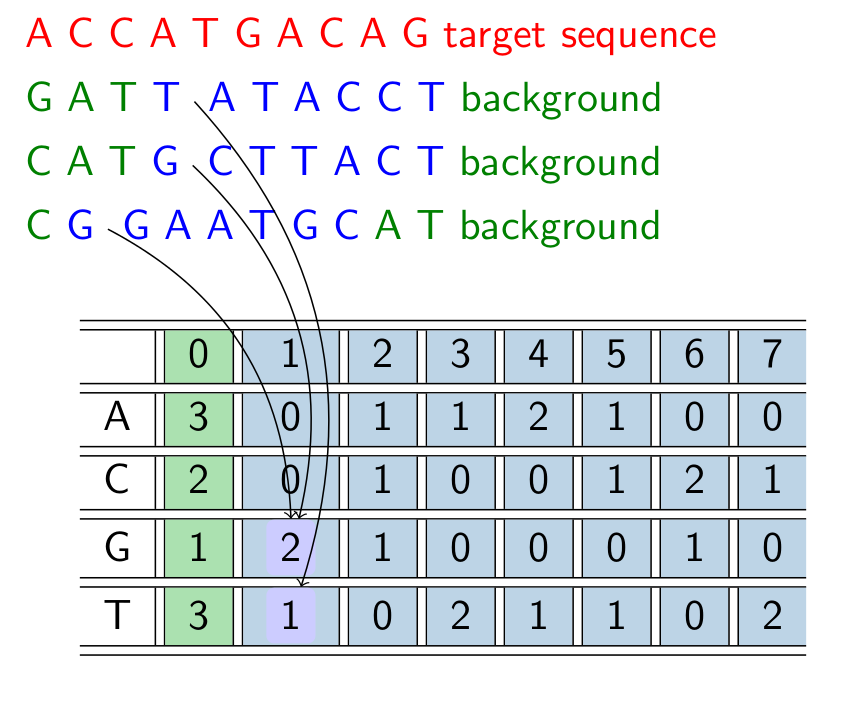
\includegraphics[width=0.7\linewidth]{GibbsTable.png}
\caption{Gibbs algorithm: creating the frequency table.}\label{gibbs1}
\end{figure}

Pseudocounts are added to the counts in the table to eliminate zeros, and counts are turned into frequencies by dividing by the number of sequences (for the blue columns) or the total number of non-motif nucleotides (for the green column).

The second part of the iteration returns to the target sequence. For each possible motif starting position in this sequence, the probability of the resultant motif is worked out using the frequency table and the following equation: 
\begin{equation}
p(M_{1}) = \frac{p_{1,A} \cdot p_{2,C} \cdot p_{3,C} \cdot p_{4,A} \cdot p_{5,T} \cdot p_{6,G} \cdot p_{7,A}}{p_{A} \cdot p_{C} \cdot p_{C} \cdot p_{A} \cdot p_{T} \cdot p_{G} \cdot p_{A}}
\end{equation}
Each element in the numerator is found by referencing the corresponding motif position (column) and nucleotide (row) in the table (Figure \ref{gibbs2}). Each element in the denominator is found by referencing the corresponding nucleotide in the zero column, irrespective of position. The lower table displays the values calculated for each of the four possible motif starting positions.  

\begin{figure}[!htbp]
\centering
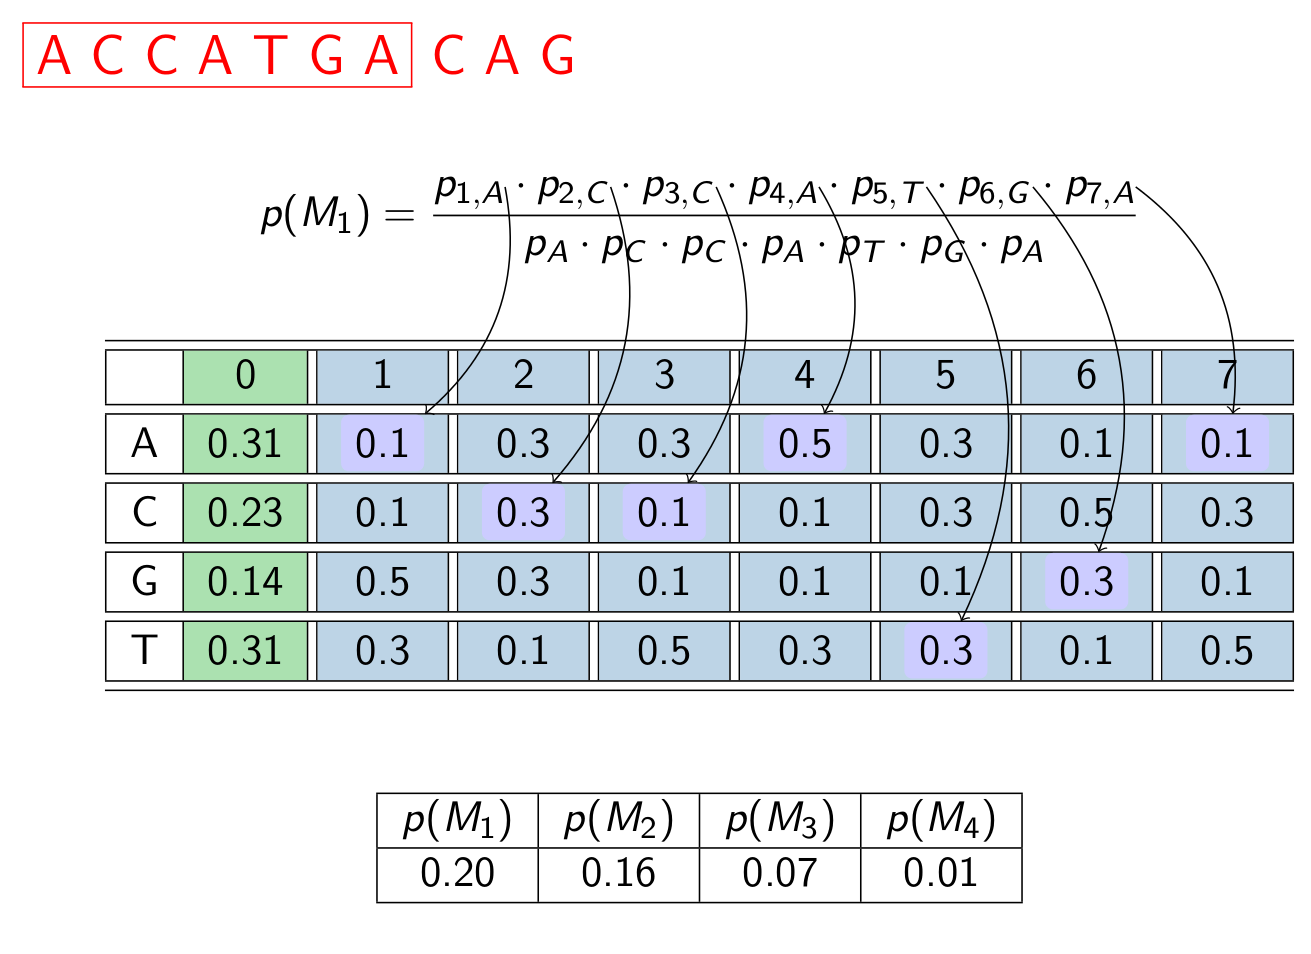
\includegraphics[width=0.7\textwidth]{GibbsTable1.png}
\caption{Gibbs algorithm: calculating the probability of the first motif start position.}\label{gibbs2}
\end{figure}

The lower table of motif probabilities is normalised, and then used to weight a random choice of motif start position for the target sequence. This choice of motif for the target sequence is the culmination of this iteration. After hundreds of such iterations, depending on the number of sequences, motif positions will no longer be totally random, but most will have been weighted according to the procedure described above. After a certain number of iterations, a log likelihood of the probability of the current set of motifs is taken. If this log-likelihood is better than the previous, it is retained; otherwise it is discarded and the algorithm returns to the motif positions for the previous log-likelihood. After many thousands of iterations the log-likelihood is never better than the previous; at this point convergence has been reached and a position weight matrix can be calculated for the set of motifs found.

The PWM itself is a useful tool that ensures that no information is lost with respect to the consensus motif sequence, since it records the frequency of each nucleotide in each position over all sequences (the position frequency matrix) before working out the probabilities for the final PWM. Another advantage is its convenient visualisation as a sequence logo, and a number of data bases (e.g. JASPAR \citep{Khan2018}; Hocomoco \citep{Kulakovskiy2018} and UniPROBE \citep{Hume2015}) now store many hundreds of PWMs that match every known transcription factor. In fact the PWM \textit{is} the motif, rather than the consensus sequence. Table \ref{pwmTable} provides an example of a PWM for the transcription factor `SP1'(using JASPAR profile MA0079 \citep{Khan2018}) and Figure \ref{pwm} provides a sequence logo for this TF that has been created from the same PWM \citep{Khan2018}.

\begin{table}[!htbp]
\centering
\caption{PWM for the SP1 transcription factor}
\label{pwmTable}
\begin{tabular}{c c c c c c c c c c c}
A & 1 & 2 & 0 & 0 & 0 & 2 & 0 & 0 & 1 & 2\\
C&1&1&0&0&5&0&1&0&1&0\\ 
G&4&4&8&8&2&4&5&6&6&0\\
T&2&1&0&0&1&2&2&2&0&6\\
\end{tabular}
\end{table}

\begin{figure}[htbp]
\centering 
     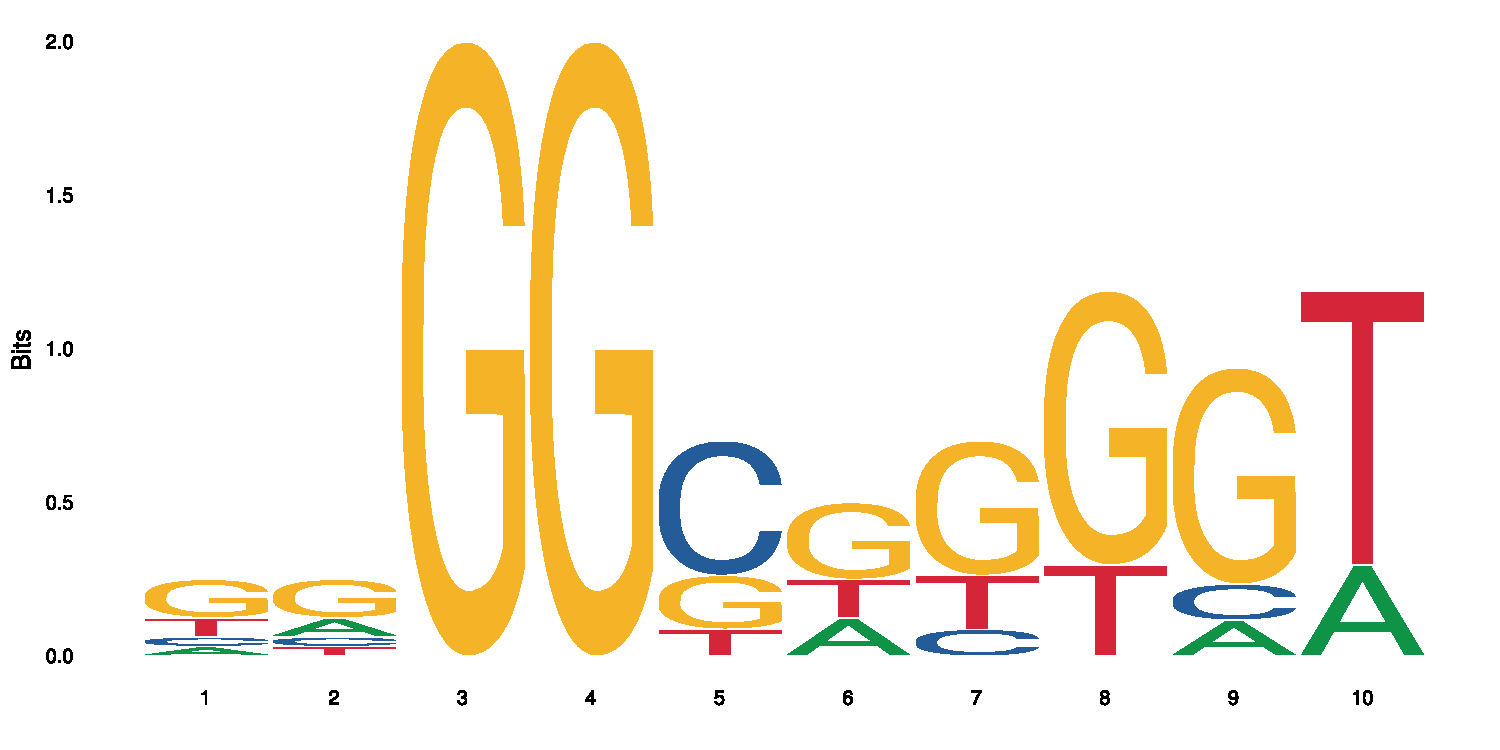
\includegraphics[width= 0.4\textwidth]{SP1Logo.pdf} 
    \caption{Sequence logo for SP1 \citep{Khan2018}.} 
    
    \label{pwm}
\end{figure}

The main disadvantage of the PWM is its assumption of independence of each position within the binding site, which may not always be true \citep{Jayaram2016}. However, as \citet{Jayaram2016} points out, in practice, PWM models tend to perform as well as more complex models that attempt to include nucleotide interdependencies in their calculations, but which are often more prone to learning noise.

\section{The Pilot Study}
\subsection{Introduction to the Pilot Study}
Computationally efficient algorithms were required for this analysis and thus a possible set of highly-used algorithms were evaluated via a pilot study using a set of 201 base pair regions with the full set of \emph{cis}- and \emph{trans}-eQTLs summary statistics generated in the CAGE study. The results from the pilot study were used to guide a larger investigation into the expected frequencies of detected motifs across the \emph{cis} sequences, and aid in the choice
of a set of algorithms for use in the main study.


\subsection{Organisation of the data}

The purpose of the pilot study was to investigate the possible methods for the identification of motifs associated with eQTLs identified by  \citet{lloyd2017genetic}. The summary statistics for the set of independent eQTL detected in the CAGE analysis were downloaded from
the CAGE browser (\texttt{http://cnsgenomics.com/shiny/CAGE/}), which contained the base pair information for each of the detected eQTL. Short target sequences of 201 base pairs, centred on the independent eQTL position (both \emph{cis} and \emph{trans}) from the CAGE analysis, formed a set of 13,930 sequences for the pilot investigation. These sequences were constructed in the R programming language \citep{rcore} using package `BSgenome.Hsapiens.UCSC.hg19' \citep{teamTBD2014}, and the \texttt{getSeq} R function \citep{durinck2005biomart}. This package references the Genome Reference Consortium Human Build 37 (GRCh37) \citep{Lander2001}, also known as hg19. Using the UCSC Table Browser \citep{karolchik2004ucsc} as a reference, these sequences were then divided into four subsets according to their location in the genome: exons; introns; promoters; and intergenic. This division into smaller subsets reduced running time within each class. Table \ref{freqComparisons} provides the number of target sequences that overlapped with these classes. Where a sequence overlapped with more than one class, it was included in both groups; hence the figures add up to more than the 13,930 sequences.

Discriminative algorithms search for motifs that are overrepresented in target sequences compared to background sequences. Since such motifs may account for the increased expression of genes associated with the target eQTLs, a discriminative approach seems ideally suited to this project.  Therefore, to identify motifs using discriminative algorithms we needed to define a background set of sequences or ``null sequences''. For this set, sequences were centred on a set 17,226 variants taken at random from the set of variants in the CAGE study that had no evidence for an effect on gene expression i.e., their association $p$-value was $>$ 0.5. Sequences of 201 base pairs surrounding these variants were again taken from the GRCh37 genome build and divided into exon, intron, promoter and intergenic subclasses. The number of null sequences in each class is provided in Table \ref{freqComparisons}. 

\begin{table}[!htbp]
\centering
\caption{Comparison of counts of region classes within target and background sequences from the pilot study.}\label{freqComparisons}
\begin{tabular}{rccccc}
 \toprule[0.2em]
Class & Exon & Intron & Promoter & Intergenic & Totals\\ 
\midrule[0.1em]
Target sequences & 2131 & 7834 & 1231 & 5132 & 16328\\
Background sequences & 387 & 6886 & 256 & 10202 & 17731\\
Totals & 2518 & 14720 & 1487 & 15334 & 34059\\
\bottomrule[0.2em]
\end{tabular}
\end{table} 
\newpage

A comparison of the target and background sequence frequencies (see Table \ref{freqComparisons}) found significant differences in the numbers for each class across target and background sequences ($\chi^2$ = 3532.8, $p$-value $<$ 0.00001). Comparatively few of the null variants fell into exon or promoter sequences, but almost twice as many null variants compared to eQTLs fell into intergenic sequences. There was little difference between nulls and eQTLs with respect to the likelihood that they might be within an intron sequence.


 
\subsection{Potential motif algorithm set}

The primary motivation of the pilot study was to establish a viable set of algorithms that could be used in the larger study. An initial literature review provided some insight into the types of algorithms that can be used to identify motifs computationally. The OMICTools directory \citep{henry2014omictools} was used to provide a list of motif-finding algorithms. The following criteria was used as a guide to the choice of motifs:
\begin{itemize}
\item Used a discriminative algorithm (comparing frequency of motif in target sequences compared to background sequences);
\item Number of citations;
\item Represented different approaches to the motif detection problem;
\item Ease of use (some programs were very difficult to install, or were no longer maintained and wouldn't run at all); and
\item Appropriate for eQTL sequences: Some algorithms are written for specific sequence sets, such as promoters, and it is unclear whether they are generally applicable to other types of sequences. Where possible algorithms that are specifically described as broadly applicable were used.
\end{itemize}

Based on these criteria, six algorithms: DREME \citep{bailey2011dreme}, HOMER  \citep{heinz2010simple}, motifRG \citep{yao2014discriminative}, STEME \citep{reid2011steme}, BaMM!motif \citep{siebert2016bayesian} and DECOD \citep{huggins2011decod}  were eventually chosen for comparison. A brief overview of each motif is provided in Appendix A.

Each algorithm provides a measure of each detected motif's enrichment, which evaluates the frequency of the detected motif in the target sequences compared to background sequences. This measure is converted and reported as an $e$-values. The $e$-value is useful in large data sets since it offers a correction for the potentially high false discovery rate. The $e$-value offers a count of expected occurrences for the given $p$-value, calculated by multiplying ``the probability that the match might occur by chance'' (the $p$-value)  by ``the number of possible occurrences''. An $e$-value close to zero represents a likely match. When the $e$-value $< 0.01$, $p$-values and $e$-values are treated as identical \citep{NCBI2006}. Using $e$-values, the motif with the highest significance is used to create a set of non-overlapping occurrences in the set of sequences that are aligned to create a position-specific probability matrix.


Using six motif-finding algorithms with four classes of sequences meant that many motifs were produced. Manual comparison of motifs across algorithms searching for similarities amongst results became very difficult. 

The STAMP algorithm \citep{mahony2007stamp} was designed for this purpose. It has two main functions:
1. To perform motif alignment and group motifs according to similarity; and
2. To search the user's database of choice for known transcription factors with similar motifs.  STAMP provides a large number of user options including:

\begin{enumerate}
\item Alignment of motifs according to Needleman-Wunsch (global) or Smith-Waterman (local) alignment methods;
\item Alignments are based on column comparison scores calculated by one of five distance metrics: Pearson's correlation coefficient; Kullback-Leibler information content; sum of squared distances; average log-likelihood ratio; or average log-likelihood with a lower limit of -2.
\item Alignment of motifs can be gapped or ungapped with a variety of penalties imposed for gap-opening and gap-extension;
\item Users may choose to trim edges of motifs;
\item Motif multiple alignment strategies can be according to `progressive profile alignment' or `iterative refinement';
\item  Two tree building algorithms are offered: an agglomerative method (UPGMA) and a divisive method based on a self-organising tree algorithm (SOTA);
\item Five transcription factor databases are offered for motif matching.
\end{enumerate}
\subsection{Results of the pilot study}

A disparate number of motifs were detected for each algorithm, with Table \ref{motif_summary} outlining potential causes for these observed differences. The algorithms also varied in the statistical details provided to support their findings, as described in Table \ref{statisticaldetails}.

\begin{table}[!htb]
\centering
\caption{Summary of motif detection algorithm properties.}\label{motif_summary}
\begin{tabular}{p{2cm}p{5cm}p{2cm}p{6cm}}
\toprule[0.2em]
\textbf{Algorithm} & \textbf{No. of motifs option} & \textbf{Entered} & \textbf{Result}\\
\midrule[0.1em]
DREME & Required & 15 & Stops finding motifs once a minimum threshold is reached\\
HOMER & Optional & Default 25 & Finds 25 motifs for every length motif requested. Since 3 lengths were default, 75 motifs were returned\\
STEME & Required & 20 & Always finds the requested number of motifs, but often reports $e$-values (to be defined) above any useful threshold\\
DECOD & Required & 20 & Does not find requested number of motifs, but no information supplied in the documentation to explain any thresholds\\
BaMM!motif & No options & No default & No information provided regarding enrichment thresholds. Varying numbers of motifs resulted, but always with useful e-values\\
MotifRG & Optional & 20	& Has threshold minimum fraction of target/background sequences (=0.01) and minimum fold change of motif in target Vs background (=1.3)\\
\bottomrule[0.2em]
\end{tabular}
\end{table}


\begin{table}[!ht]
\centering
\caption{Comparison of statistical details for each motif detection algorithm}\label{statisticaldetails}
\begin{tabular}{p{0.1\linewidth}p{0.2\linewidth}p{0.2\linewidth}p{0.4\linewidth}}
\toprule[0.2em]
Algorithm & Enrichment Calculation & $p$-value/$e$-value provided & Other details\\
\midrule[0.1em]
DREME & Fishers Exact Test & $p$-values/$e$-values & None\\
HOMER & Cumulative binomial distribution & uncorrected $\;\;\;\;\;\;$ $p$-values & Provides the number of target and background sequences that contain the motif\\
STEME & Not provided & $e$-values & Provides target and background numbers within mass of log data (difficult to locate)\\
DECOD & $z$-values & $e$-values & $e$-values only provided for the GUI-version, not for the terminal version\\
BaMM! & Log-odds score & $e$-values & Varying numbers of motifs produced with significant $e$-values. Documentation states that threshold is $p<1.0$, but this is not reflected in results, which have very small $e$-values\\
motifRF & Wald test & Not provided & None\\
\bottomrule[0.2em]
\end{tabular}
\end{table} 


Running the algorithms on each subset of the data resulted in a set of motifs for each sequence subset. Within each subset, motifs were formatted as input for the STAMP algorithm, which performed motif alignment across all motif sets and grouped the motifs according to similarity. Default parameters were used: Pearson Correlation Coefficient for distance metrics; Smith-Waterman local alignment ungapped alignment: Iterative refinement multiple alignment; UPGMA tree building; and the JASPAR database \citep{sandelin2004jaspar} to identify those motifs that corresponded to a known transcription factor.  

No strong differences emerged in the results from the four groups (exon, intron, promoter, and intergenic). Since the purpose of the pilot study was to evaluate the algorithms, rather than to do an in depth study of motifs found and associated transcription factors, a brief summary will be provided of results from one group only: the exon set of sequences. 

The six different algorithms returned a total of 770 motifs in the exon sequences, illustrated in the circular cladogram developed using Evolview tree viewing software  \citep{He2016}. Although the number of motifs means that the labelling on the cladogram is not easily distinguishable, the colouring provides an illustration of the number and spread of motifs found by each algorithm (Figure \ref{fig: exon_cladogram}). In the exon sequences, HOMER found the most motifs, with good variability. STEME, DECOD and DREME also achieved a good spread, but reported relatively few motifs. However, in the case of DREME, this paucity of motifs seemed to be due to the use of the website rather than the downloaded version of the motif finding tool, since a later check using the downloaded version returned a large number of motifs. BaMM!motif also achieved a good spread of a large number of motifs. RGMotif did not perform well, with only a few motifs all clumped together, bearing no relationship to motifs found by other algorithms.

\begin{figure}[htbp] 
     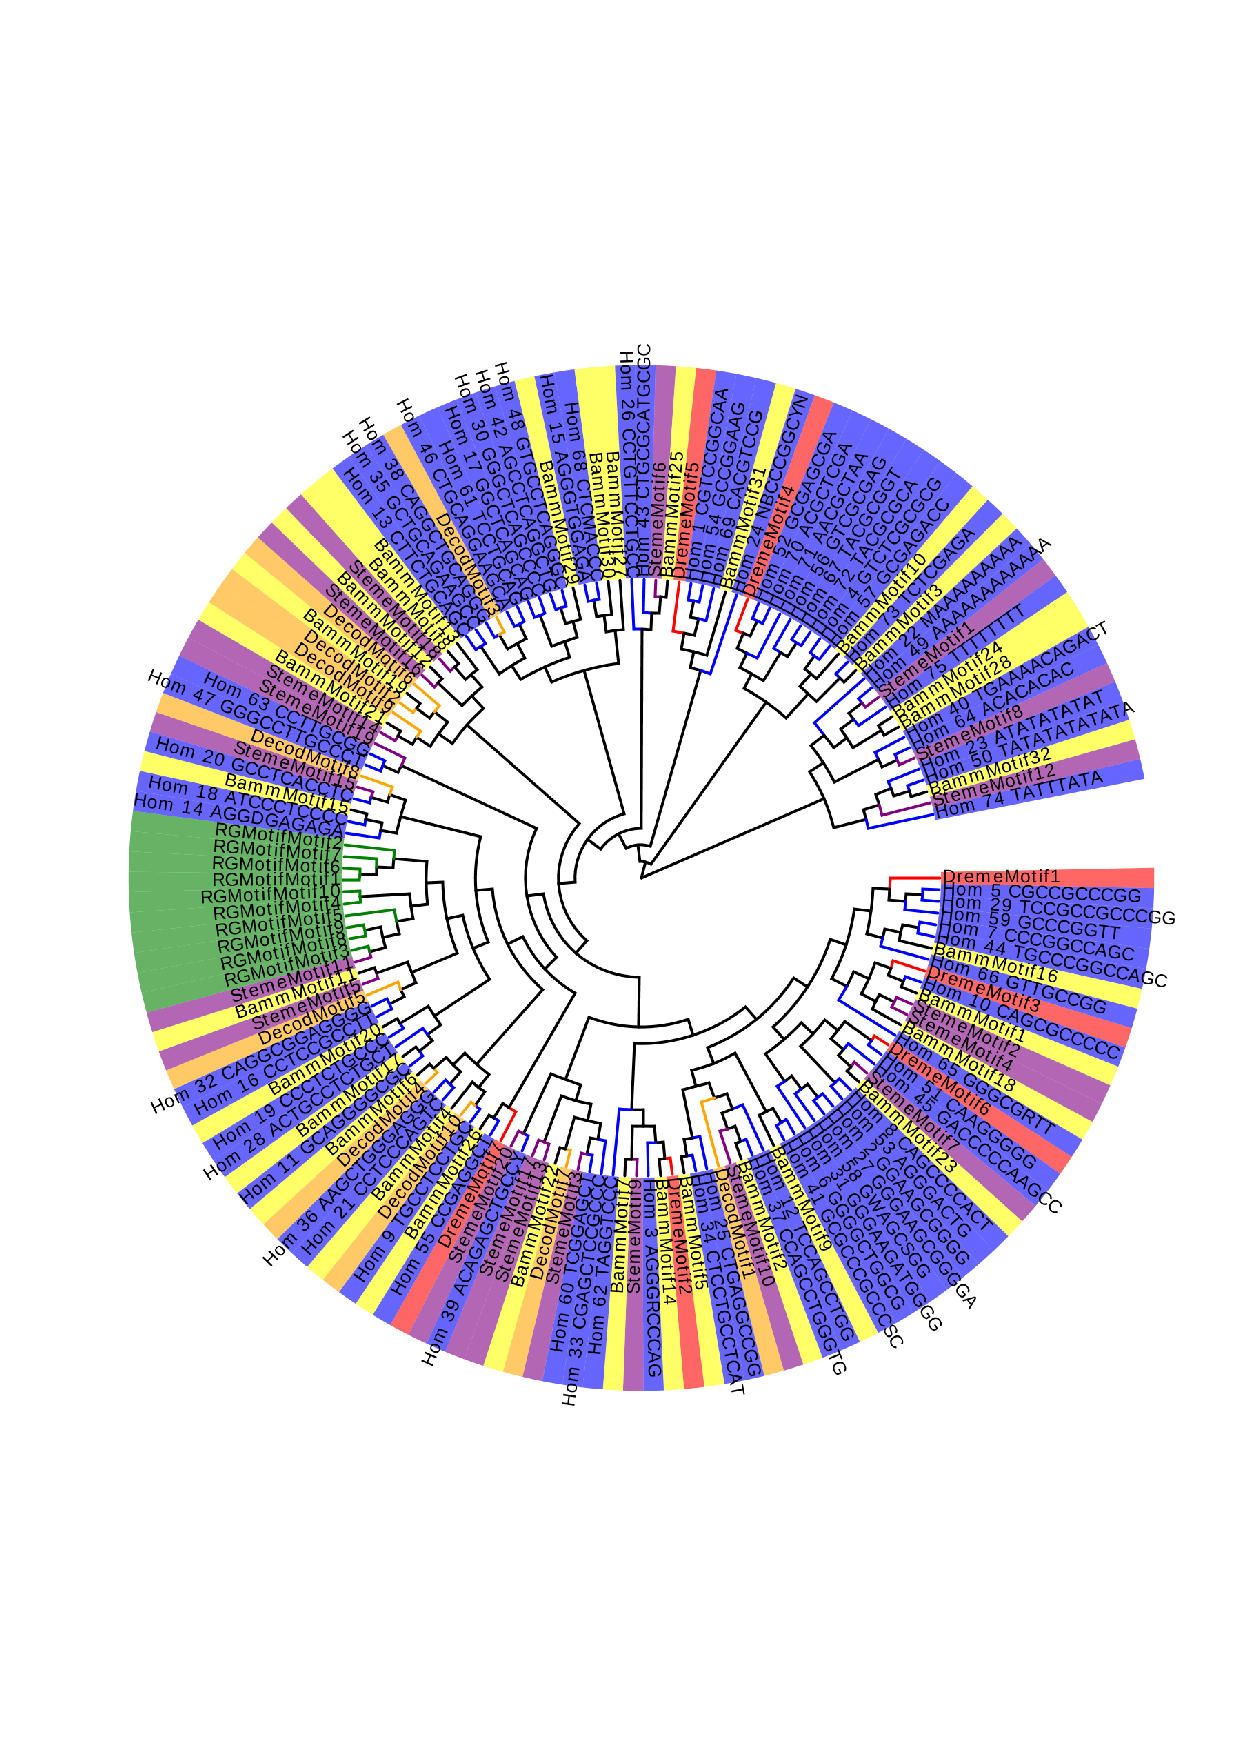
\includegraphics[width= \textwidth]{exon_pilot_cardiogram.pdf} 
    \caption{{\bf Circular cladogram of 770 exon motifs from Evolview tree viewing software \citep{He2016} }. 
    The cladogram depicts motifs detected from DREME (red), HOMER (blue), BaMM!motif (yellow), MotifRG (green), STEME (purple)
    and DECOD (orange). Motifs closer in the plot have motif sequences that are more similar.}
    \label{fig: exon_cladogram}
\end{figure}

Using the JASPAR data base, the STAMP algorithm was able to match all of the motifs as potential binding sites for transcription factors. It is often the case that a single transcription factor has many different binding motifs. For this reason the 770 motifs were identified as binding sites for 99 transcription factors, with more than half the motifs identified as potential binding sites for a subset of just 17 transcription factors, as illustrated in Table \ref{fig: motif_tf_summary_exons}. 


\begin{table}[!ht]
\centering
\caption{Summary of transcription factor (TF) matches to motifs detected in exonic sequences in the pilot study}\label{fig: motif_tf_summary_exons}
\begin{tabular}{p{0.3\linewidth}p{0.3\linewidth}p{0.3\linewidth}p{0.4\linewidth}}
\toprule[0.2em]
Transcription factor motif & Matching motifs & Cumulative sum\\ 
\midrule[0.1em]
E74A & 38 & 38 \\
Snail & 33 & 71\\
TFAP2A & 33 & 104\\
ABI4 & 32 & 136\\
SP1 & 29 & 165\\
SPIB & 23 & 188\\
ZNF42{\_}1-4 & 22 & 210\\
Roaz & 21 & 231\\
GABPA & 20 & 251\\
ELK4 & 19 & 270\\
Myf & 18 & 288\\
TEAD & 18 & 306\\
E2F1 & 17 & 323\\
Klf4 & 16 & 339\\
SP11 & 16 & 355\\
NHLH1 & 15 & 370\\
Pax4 & 15 & 385\\
\bottomrule[0.2em]
\end{tabular}
\end{table} 
\newpage
It should be noted that the $p$-values for these matches were not subjected to any multiple testing correction. Please note that the reference to $p$-value here describes a measure on the 'match' of a particular motif to a transcription factor and not the enrichment $p$-value from the motif detection analysis.
In the larger study, this correction was implemented, resulting in a much smaller number of matched motifs and a large number of motifs unmatched to a transcription factor.

Enrichment values for motifs found in eQTL sequences compared to the null sequences are provided in Table \ref{motif_evalue_summary_exons}. These enrichment values are reported as $e$-values by all algorithms apart from HOMER, whose enrichment values are reported as $p$-values. As mentioned previously, if an $e$-value $< 0.01$, the $e$-value is considered to be identical with the $p$-value \citep{NCBI2006}. As illustrated, many values found by STEME (high $e$-values) are at odds with those found by other algorithms. As mentioned previously, RGmotif did not provide enrichment values and so is missing from this table. 

\begin{table}[!ht]
\centering
\caption{TFs found by all algorithms with associated enrichment $e$-values, ordered by DREME $e$-values in pilot exon sequences (NMF = no motif found)}\label{motif_evalue_summary_exons}
\begin{tabular}{p{0.15\linewidth}p{0.15\linewidth}p{0.15\linewidth}p{0.15\linewidth}p{0.15\linewidth}p{0.17\linewidth}}
\toprule[0.2em]
Exon TF & Homer $p$-value & Dreme $e$-value & Steme $e$-value & Decod $e$-value & BaMM!motif $e$-value\\ 
\midrule[0.1em]
E74A      	&1.00$\times10^{-155}$	&1.80$\times10^{-4}$	&6.77$\times10^{+259}$	&1.50$\times10^{-3}$	&4.84$\times10^{-34}$\\
Snail      	&1.00$\times10^{-85}$	&1.70$\times10^{-2}$	&1.12$\times10^{+33}$	&1.35$\times10^{-3}$	&5.99$\times10^{-36}$\\
TFAP2A	&1.00$\times10^{-96}$	&1.30$\times10^{-21}$	&6.69$\times10^{+22}$	&2.65$\times10^{-3}$	&1.31$\times10^{-43}$\\
ABI4		&1.00$\times10^{-101}$	&1.30$\times10^{-21}$	&6.69$\times10^{+22}$	&1.35$\times10^{-3}$	&2.72$\times10^{-51}$\\
SP1		&1.00$\times10^{-123}$	&1.30$\times10^{-21}$	&4.43$\times10^{-10}$	&1.84$\times10^{-3}$	&4.88$\times10^{-9}$\\
SPIB		&1.00$\times10^{-128}$	&2.50$\times10^{-2}$	&1.69$\times10^{-21}$	&1.46$\times10^{-3}$	&1.42$\times10^{-35}$\\
ZNF42{\_}1-4&1.00$\times10^{-123}$	&1.30$\times10^{-21}$	&6.69$\times10^{+22}$	&1.38$\times10^{-3}$	&2.72$\times10^{-51}$\\
Roaz		&1.00$\times10^{-102}$	&1.60$\times10^{-13}$	&1.12$\times10^{+33}$	&3.74$\times10^{-3}$	&2.72$\times10^{-51}$\\
GABPA	&1.00$\times10^{-155}$	&1.80$\times10^{-4}$	&NMF					&1.50$\times10^{-3}$	&4.84$\times10^{-34}$\\
ELK4	&1.00$\times10^{-155}$	&1.80$\times10^{-4}$	&6.77$\times10^{+259}$	&1.50$\times10^{-3}$	&4.84$\times10^{-34}$\\
Myf		&1.00$\times10^{-128}$	&NMF				&1.99$\times10^{+70}$	&1.35$\times10^{-3}$	&1.74$\times10^{-27}$\\
TEAD	&1.00$\times10^{-107}$	&2.50$\times10^{-2}$	&1.69$\times10^{-21}$	&1.84$\times10^{-3}$	&9.91$\times10^{-1}$\\
E2F1	&1.00$\times10^{-101}$	&1.40$\times10^{-8}$	&1.09$\times10^{+293}$	&1.38$\times10^{-3}$	&1.74$\times10^{-27}$\\
SPI1		&1.00$\times10^{-128}$	&NMF				&1.69$\times10^{-21}$	&1.50$\times10^{-3}$	&3.31$\times10^{-5}$\\
ZNF42{\_}5-13&1.00$\times10^{-90}$&1.90$\times10^{-11}$	&4.43$\times10^{-10}$	&NMF				&5.90$\times10^{-22}$\\
TP53	&1.00$\times10^{-77}$	&1.30$\times10^{-21}$	&1.12$\times10^{+33}$	&3.74$\times10^{-3}$	&4.88$\times10^{-09}$\\
\bottomrule[0.2em]
\end{tabular}
\end{table}

No further analysis is provided of these results, as the purpose of the pilot study was to demonstrate that the algorithms are capable of detecting motifs; and secondly, to provide a basis to evaluate the algorithms with respect to their suitability for the larger scale analysis.
\newpage
The pilot study suggests that the two algorithms HOMER and BaMM!motif  have the most extensive coverage of motif binding sites. The recently published BaMM!motif algorithm is particularly impressive, given the fine tuning of its motifs, unlike HOMER, whose motifs are frequently clumped into broad clusters. Both these motif finding algorithms have high computational efficiency making them well suited to the large sequence analysis. DREME is also 
efficient, but fails to find some motifs that are found by every other algorithm. However, with further analysis, this proved to be due to the use of the website version of the software during the pilot study. The use of the downloaded version led to motif discovery comparable to the HOMER algorithm. DECOD was computationally inefficient and did not report many motifs. STEME was computationally inefficient, and reported $e$-values that differed from those reported by the other algorithms. Finally, motifRG seemed to miss many motifs and did not report the significance of those it found, which were clumped together, failing to align with any of the motifs found by other algorithms. 

On the basis of this pilot study, the algorithms chosen for the main study were HOMER, BaMM!motif and DREME.


\subsection{Moving from 200 kb sequences to larger sequences}

The pilot data looked at small regions surrounding the eQTLs. The full analysis examined much longer sequences, which increased the computational challenge relative to the pilot study.  An initial investigation was conducted to determine the most appropriate length of sequence with respect to the possibility of sequence overlap between eQTL and null sequences. The purpose of this investigation was to determine the degree of overlap between eQTL and null sequences. Substantial overlap reduces the ability of algorithms to discriminate between target and null sequences when searching for relative motif enrichment. Sequences of four different lengths: 200001 bases; 40001 bases; 10001 bases; and 2001 bases) (termed 200 kb, 40 kb, 10 kb and 2 kb sequences) were created, all centred on the eQTLs used in the pilot study. The same length sequences were also created for the variants with no effect (termed null sequences). The likelihood of overlap increases with the length of the sequence. A python program was written to isolate all overlaps. If an eQTL sequence had more than one overlap (e.g. with different null sequences overlapping the start and finish of the eQTL sequence), the largest overlap was used to calculate the size of the overlap. An R program was used to convert these overlaps into a histogram of the number of overlapping sequences as a percentage of all sequences within each chromosome.

Figure \ref{fig: 100kbOverlaps}(a) provides a histogram (by chromosome) of the percentage of eQTL sequences that overlapped with null sequences for the 200 kb sequences. As illustrated, a majority of chromosomes had at least 40 percent of their sequences with some degree of overlap, with close to 80 percent of sequences in three chromosomes overlapping with null sequences. Figure \ref{fig: 100kbOverlaps}(b) illustrates the percentage of sequences within each chromosome that overlapped by at least 50 percent of sequence length. Twenty percent of sequences in almost every chromosome fell into this category, and for chromosome 13, sixty percent of sequences had at least 50 percent overlap.


\begin{figure}[!htbp]%
\centering
\subfloat[All 200 kb sequences with overlap]{{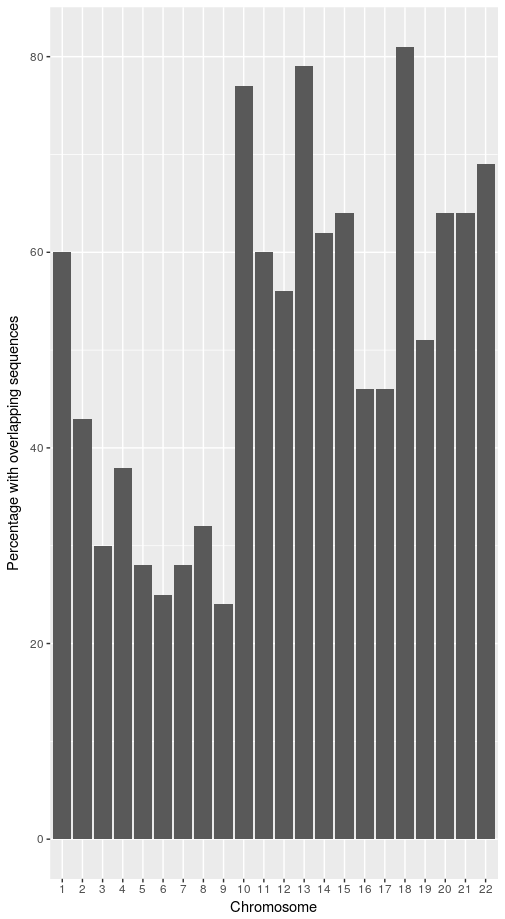
\includegraphics[width=0.4\textwidth]{100kbOverlapCount.png} }}%
\qquad
\subfloat[200 kb sequences with 50 percent overlap]{{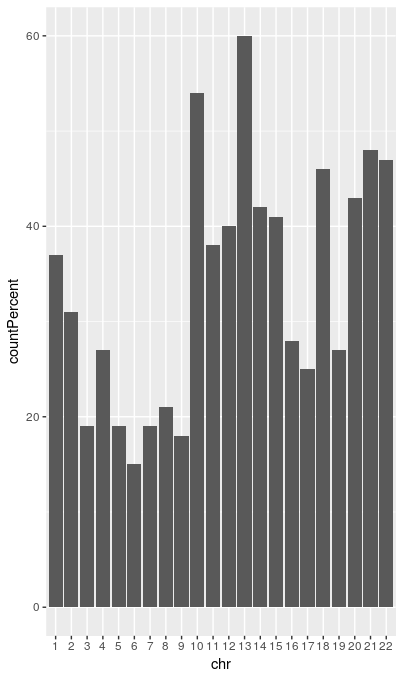
\includegraphics[width=0.4\textwidth]{100kbSequencesWith50PercentOverlap.png} }} 
\caption{Summary of overlap percentage of eQTL and null sequences for 200 kb sequences with overlaps.}
\label{fig: 100kbOverlaps} 
\end{figure}  


For 40KB sequences, the percentage of eQTL sequences that overlapped with null sequences by chromosome, with no account taken of the size of the overlap, 
was approximately 20 percent. Only one chromosome had more than 30 percent of sequences overlapping with null sequences, although all chromosomes had at least ten percent of their sequences with some overlap. Only one chromosome had more than 15 percent of its sequences with 50 percent overlap or more. For 10 kb sequences, the overlap is substantially reduced. A maximum of eight percent of sequences in any chromosome experience any overlap with on average 
four percent of the sequences having overlap greater than 25 percent on average across the genome.

Finally, Figure \ref{2kbOverlaps} illustrates the amount of overlap when sequence length is restricted to 1000 bases on either side of the variant (2 kb sequences). Figure \ref{2kbOverlaps}(a) shows the percentage of all overlaps (of any length) within each chromosome, and Figure \ref{2kbOverlaps}(b) shows the percentage of sequences that overlap by at least 25 percent. As shown in this figure, almost all chromosomes have only 1 or 2 percent overlapping sequences, and only 1 or 2 percent overlap by more than 25 percent.

\begin{figure}[!htbp]%  
\centering
\subfloat[All 2 kb sequences with overlap]{{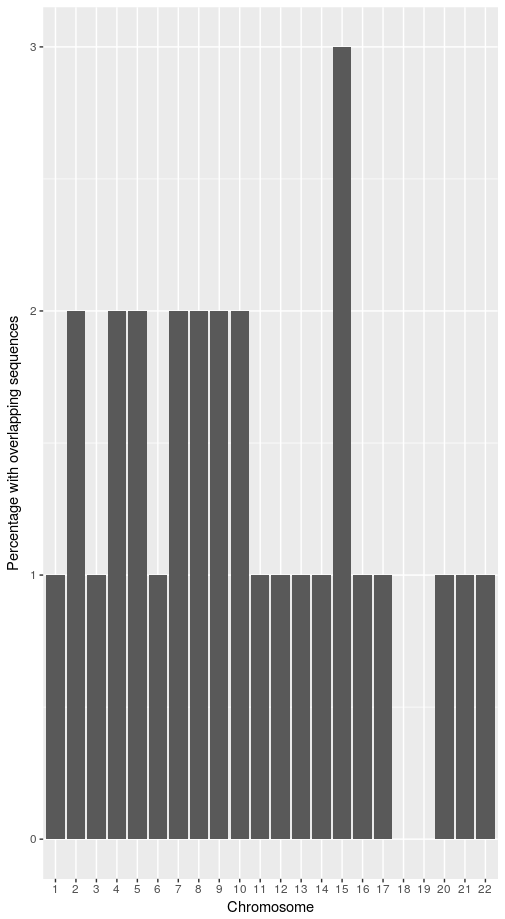
\includegraphics[width=0.4\textwidth, height=0.7\textwidth]{1kbSequenceOverlap.png} }}% 
\qquad
\subfloat[2 kb sequences with 25 percent overlap]	{{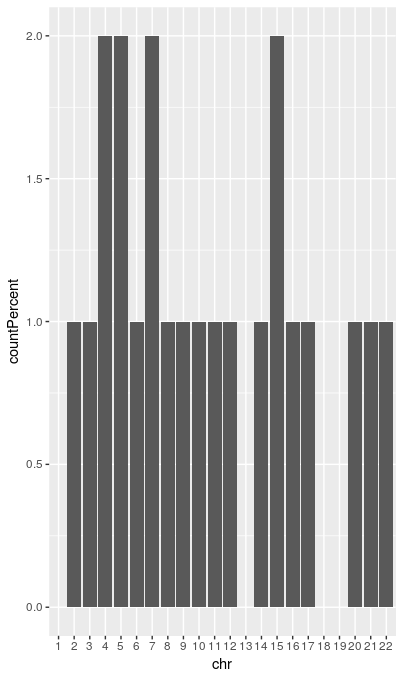
\includegraphics[width=0.4\textwidth, height=0.7\textwidth]{1kbSequences25PercentOverlap.png} }}
\caption{2 kb sequence overlap between null and eQTL sequences.} \label{2kbOverlaps}%
\end{figure}  

This analysis indicated that using sequences of length 2001 base pairs is a good compromise that both maximised computational efficiency and minimised sample overlap.
 

\section{Large scale study} 
\subsection{Materials and methods}

The main study used HOMER  \citep{heinz2010simple}, BaMM! \citep{siebert2016bayesian} and DREME \citep{bailey2011dreme} motif algorithms to analyse 10,499 genomic sequences centred at the \emph{cis}-eQTLs discovered in \citet{lloyd2017genetic}. Only the \emph{cis}-eQTL were used in the main study as  \emph{cis} gene regulation is better understood relative to  \emph{trans} regulation in the genomics literature. As this was an
exploratory study, the uncertainty around the action of \emph{trans} gene regulation would have added a further complexity, although it warrants scientific
investigation. The null sequences were generated using 2 kb sequences centred around a random sample of 10,499 null variants from the \citet{lloyd2017genetic} gene expression study. 

As for the pilot study, all sequences were constructed using the hg19 reference genome \citep{Lander2001}. An R program was written drawing on sequence information provided by the `BSgenome.Hsapiens.UCSC.hg19' package \citep{bsghg19}. Because \emph{cis}-eQTLs can regulate more than one gene the original 11,204 \emph{cis}-eQTLs contained repeats; resolving these led to 10,499 \emph{cis}-eQTLs for sequence construction. The same number of null sequences, centred on a random selection of non-eQTL variants, were also produced. The R program created \texttt{bed} files, which were used for HOMER annotation data, and \texttt{fasta} files, which were used as target and background by the motif finding algorithms.

The following section details the parameters that were used as input for each of the algorithms, and the output of the algorithm.
\newpage
\subsubsection{Detailed description of application of DREME, HOMER and  BaMM!motif algorithms}



\paragraph{DREME parameters and output}\mbox{}\\
DREME runs from the terminal using the following command:

\texttt{/usr/bin/dreme[options]}

Options used were:
\begin{itemize}
\item the specified output directory (overwriting if necessary);
\item the positive sequence file; 
\item the negative sequence file
\end{itemize}
The default motif $e$-value of 0.05 was used as the threshold.

As output, DREME provides two main files: the PWM file of motifs, and an html file listing all motifs as sequence logos, with both an $e$-value and an `unerased' $e$-value which is calculated without erasing sites of previously found motifs. The html file provides further information which includes the number of target and background sequences that contain the motif, together with the corresponding $p$-value and $e$-value (calculated by multiplying the $p$-value by the number of motifs found). The $p$-value was calculated for each motif using Fisher's Exact Test for enrichment of the motif in the positive sequences.

As part of the MEME suite, DREME provides opportunity to submit the motif(s) to other algorithms within the MEME suite. These other algorithms include: `Tomtom', which will search for similar known motifs; `MAST' and `FIMO' which will search sequences for known motifs and provide enrichment details; `GOMO' which will identify Gene Ontology terms for the motif; and `SpaMo' which will search for possible transcription factor complexes.

\newpage
\paragraph{HOMER parameters and output}\mbox{}\\
HOMER can use both bedfiles and fasta sequences. With fasta sequences HOMER runs from the terminal using the following command:

\texttt{findMotifs.pl $<$positive sequence file$>$ fasta $<$output directory$>$ -fasta $<$negative sequence file$>$ [options]}
 
 
Options used were:
\begin{itemize}
\item -mask: mask motifs once found, as well as oligos immediately adjacent to the site that overlap with at least one nucleotide.
\item -len 4,5,6,7,8,9,10,11,12,13,14 : find motifs of these lengths
\end{itemize}
The number of motifs per length requested (default=25), plus the length of the oligo seeds (default=1,2,3), were left at default.

An important time saving feature used by the HOMER algorithm is an initial scan of the sequences using HOMER's data bank of known motifs that match to transcription factors. Scanning for known PWMs is much faster than searching for motifs de novo, and any matches that are found can be masked from the sequences, thereby reducing the search space for the de novo search. All motifs found in this initial scan are placed in a folder named `knownResults' as a set of sequence logos.

HOMER also normalises its oligo enrichment counts according to the `ATGC' content of each oligo. A file with the extension `.autonorm.tsv' provides details of overall nucleotide content and the normalisation factor for each oligo.

The full set of motifs found by HOMER is provided in a file with the extension `.all.motifs'. In this file, the PWMs are organised firstly by length, secondly by $p$-value. The default number of motifs found per motif length is 25. Given that motifs were requested for fourteen different lengths i.e. 4, 5, 6, 7, 8, 9, 10, 11, 12, 13, and 14, the file contained $14 \cdot 25 = 350$ PWM's. Each PWM begins with a header such as: 


$>$ATGATTCAATTACC	114-ATGATTCAATTACC	
10.16267	-42.58457	0.0\\	T:666.0(6.34\%), B:378.0(3.67\%), P:1e-18\\ Tpos:1015.5, Tstd:559.1, Bpos:988.7, Bstd:749.1, StrandBias:0.1, Multiplicity:1.05
\begin{itemize}
\item $>$ + Consensus sequence 
\item Motif name (usually the same as the consensus sequence)
\item Log odds detection threshold, used to determine bound vs. unbound sites 
\item $\log(p$-value) of enrichment
\item 0.0  A place holder for backward compatibility
\item Occurrence Information separated by commas, including:
\begin{itemize}
\item T: number of target sequences with motif, \% of total of total targets
\item B: number of background sequences with motif, \% of total background
\item P: final enrichment $p$-value
\end{itemize}
\item Motif statistics separated by commas: 
\begin{itemize}
\item Tpos: average position of motif in target sequences (0 = start of sequences)
\item Tstd: standard deviation of position in target sequences
\item Bpos: average position of motif in background sequences (0 = start of sequences)
\item Bstd: standard deviation of position in background sequences
\item StrandBias: log ratio of + strand occurrences to - strand occurrences.
\item Multiplicity: The average number of occurrences per sequence in sequences with 1 or more binding sites.
\end{itemize}
\end{itemize}

HOMER also tries to match each de novo motif found using its data bank of transcription factors, and provides a number of files describing the statistical details of each matched motif with its possible transcription factor.

HOMER has an extensive set of webpages describing different ways in which its algorithms can be used. This includes a caution that only motifs that are `very enriched' should be considered to be robust - HOMER uses a cumulative binomial distribution to calculate $p$-values and suggests a threshold $p$-value $ <1\times10^{-50}$ for robust significance. This threshold was adopted throughout this project. 

As described above, the motif header in the PWMs provides the average position of the motif together with its standard deviation. Further information can be recovered using another tool that is part of the HOMER software. The `annotatePeaks.pl' command has options that can be used to recover general genomic information about the set of sequences, as well as the specific position of the motif in each sequence. An option that was used in this project is the `-hist' option, which provides data that can be used to create a graph of the distance of the motif from the centre of the sequence over the set of 10,499 sequences.

\paragraph{BaMM!motif parameters and output}\mbox{}\\
BaMM!motif runs from the terminal using the following command:

\texttt{BaMMmotif $<$output directory$>$ $<$positive sequence file$>$ [options]}

Options used were:
\begin{itemize}
\item --negSequenceSet: the set of null sequences
\item --reverseComp: use both strands of dna (this was default for both DREME and HOMER)
\item --maxPValue: the maximum $p$-value of the PWMs (The maximum P-value was changed from the default of 1 to $p<0.05$, but applying this option seemed to have no affect on the results obtained)
\end{itemize}

As output BaMM!motif provides a set of matrices which the writers of the algorithm suggest be referred to as a set of `BaMMs' rather than PWMs. Each `BaMM' is preceded by a header listing the number of target sequences containing the motif and the $e$-value. This file follows the standardised MEME formatting so that it could be submitted directly to the MEME suite for further processing if desired.

In addition to the `BaMM' file, the BaMM!motif algorithm provides a PWM file created using a zero order Markov model. It provides a `MotifFile.txt' which lists each motif as a sequence, together with its $e$-value and the number of target sequences containing the motif (this is the same information as is provided in the header to each `BaMM'). A very long file (with the extension `Pvals.txt') lists, for every motif, each sequence that contains the motif (as a sequence number), the start position of the motif in the sequence, the strand (+ or -) and the $p$-value of the individual motif in the sequence. The $p$-values were calculated using the log-odds score calculated by dividing the probability of the motif in the positive sequences by the probability of the motif in the background sequences \citep{siebert2016bayesian}. Finally, another file with the extension `sequence.txt' provides a key that links the sequence number listed in the `Pvals.txt' file to the relevant eQTL provided in the original fasta file submitted to the algorithm. 

\subsubsection{Computer resources}

All algorithms were run and computations performed on a personal computer (Dell Latitude E6320 with 8GB RAM; Intel Core i5-2520M CPU @2.50GHz x 4). Calculation of run times are provided as approximates, since the algorithms were run several times with different parameters and data. The approximate run times for the algorithms were as follows:
\begin{itemize}
\item HOMER: took approximately 6 hours and required no extra memory. Other tasks could be performed whilst HOMER ran in the background.
\item DREME: took approximately 15 hours and required no extra memory, but other tasks were slowed down considerably.
\item BaMM!motif: took approximately 8 hours to produce almost all the data, but then an extra 24 hours to produce the final log likelihood. This was not necessary information, so the program was concluded manually (using `Control+C') once all other files were produced. The program required an extra 32GB of virtual memory, and no other tasks could be performed whilst it was running.
\end{itemize}


\subsubsection{Validation of algorithm results}

One concern with the use of computational methods for de novo motif detection is the proportion of false positives. For example, a motif may not be enriched relative to the background but the significant enrichment is instead a result of unaccounted for confounding, convergence to a particular unwanted motif optimum, or poor control for multiple testing. To investigate the potential of each algorithm to report false positives the following initial checks were performed:
\begin{enumerate}
\item Two types of analysis were performed with respect to the null sequences:
\begin{enumerate}
\item The first analysis used the algorithms to check whether the null sequences contained any motifs that were enriched in the null sequences compared to the eQTL sequences. It was expected that few, relatively unimportant, motifs would be found. This analysis was formed under the biological hypothesis that motifs are more likely to be harboured close to functional parts of the genome, which may be false.
\item The second analysis was a more genuine check of the algorithms' capacity to report false positives. After a random split of all null sequences into two groups, each algorithms checked for enriched motifs in the first group compared to the second group. It was expected that the two groups would be generally similar and that no motifs would be found. 
\end{enumerate}
\item A further check used the AME algorithm \citep{Buske2010} to provide enrichment values for all significant motifs found by the DREME, HOMER and BaMM!motif algorithms. 
\end{enumerate}

\subsubsection{Analysis of the algorithm results}

The motif files were formatted and subjected to the STAMP algorithm, which performed the following procedure:
\begin{enumerate}
\item Alignment of motifs
\item Creation of a cladogram to illustrate motif similarity
\item Matching of motifs to transcription factors using the JASPAR data base \citep{Mathelier2016}
\end{enumerate}

A number of programs (both in Python and R) were written and incorporated into scripts to further process these initial results, as described in Results. HOMER's annotation algorithm was also used to calculate occurrence and average distance from the variant (both eQTL and null) across all motifs and sequences. To measure the occurrence of each motif in each sequence, the following command was used to access HOMER annotation software:

\texttt{annotatePeaks.pl $<$eQTL sequences as a bedfile$>$ hg19 -m $<$motif PWM file$>$ $>$ $<$result file$>$ -nmotifs -mdist -noann}

To provide a list of average distances from the centre for all motifs, the following command was used:

\texttt{annotatePeaks.pl $<$eQTL sequences as a bedfile$>$ hg19 -m $<$motif PWM file$>$ $>$ $<$result file$>$ -hist 100 -noann}


\subsection{Results}

Table \ref{eQTLmotifNumbers} provides the results of all three algorithms with respect to the total number of motifs found that were enriched in eQTL sequences compared to null sequences, as well as the number of motifs that met the stringent cut-off of $p$-value$<1\times10^{-50}$.



\begin{table}[!htbp]
\caption{Motifs enriched in eQTL sequences compared to null sequences.}
\label{eQTLmotifNumbers}
\centering
\begin{tabular}{ccccccc}
\toprule[0.2em]
\multicolumn{3}{c}{All motifs} & & \multicolumn{3}{c}{Motifs with $p$-value$<1\times10^{-50}$}\\
\cmidrule[0.1em]{1-3}
\cmidrule[0.1em]{5-7}
DREME & HOMER & BaMM!motif && DREME & HOMER & BaMM!motif\\
114 & 238 & 99 && 44 & 141 & 38\\
\bottomrule[0.2em]
\end{tabular}
\end{table}

A visual examination of the large number of HOMER motifs found that some of the smaller motifs were subsets of the larger motifs. Although masking prevents motif repetition during a single search, the masking is removed for a new search for a motif of a different length. After all motif subsets within the HOMER motifs were removed, the number of significant HOMER motifs was reduced from 141 to 123.

Before further analysis of these motifs was conducted, validation of algorithms was conducted using the null sequences. The first check was a search for motifs that were enriched in the null sequences compared to the eQTL sequences. Results of this search are provided in Table \ref{nullMotifNumbers}:

\begin{table}[!htbp]
\caption{Motifs enriched in null sequences compared to eQTL sequences.}
\label{nullMotifNumbers}
\centering
\begin{tabular}{ccccccc}
\toprule[0.2em]
\multicolumn{3}{c}{All motifs} & & \multicolumn{3}{c}{Motifs with $p$-value$<1\times10^{-50}$}\\
\cmidrule[0.1em]{1-3}
\cmidrule[0.1em]{5-7}
DREME & HOMER & BaMM!motif && DREME & HOMER & BaMM!motif\\
103 & 235 & 278 && 39 & 0 & 168\\
\bottomrule[0.2em]
\end{tabular}
\end{table}

HOMER returned a large number of motifs, but none of them met the stringent cut-off threshold. DREME found approximately the same number of motifs in the null sequences as in the eQTL sequences, and BaMM!motif found many more (168 significant motifs in the null compared to 38 in the eQTL sequences). The results from DREME and BaMM!motif algorithms provide evidence to contradict the hypothesis that null sequences do not harbour motifs. 


The BaMM!motif results in the second check show a further unexpected result, where BaMM!motif reported motifs in the null Group A versus null Group B analysis. It was expected that the algorithms should find few significant motifs in this analysis (Table \ref{nullHalfGroups}).

\begin{table}[!htbp]
\caption{Motifs enriched in null Group A compared to null Group B}
\label{nullHalfGroups}
\centering
\begin{tabular}{ccccccc}
\toprule[0.2em]
\multicolumn{3}{c}{All motifs} & & \multicolumn{3}{c}{Motifs with $p$-value$<1\times10^{-50}$}\\
\cmidrule[0.1em]{1-3}
\cmidrule[0.1em]{5-7}
DREME & HOMER & BaMM!motif && DREME & HOMER & BaMM!motif\\
0 & 55 & 237 && 0 & 0 & 132\\
\bottomrule[0.2em]
\end{tabular}
\end{table}

The results for both DREME and HOMER in null Group A versus null Group B analysis suggest that the proportion of false positives, expected at the chosen significant thresholds, is negligible (Table \ref{nullHalfGroups}). DREME found no motifs, whilst HOMER found some motifs at a very low level of significance ($p$-value $>1\times10^{-8}$). However, BaMM!motif reported a larger number of motifs. Given this result, the test was repeated for the BaMM!motif algorithm, reversing the groups. BaMM!motif found a similar number of motifs significantly enriched in Group B compared to Group A. Furthermore, the most highly enriched motif for Group A (CTACTAAAAATACAAAA) is also the most highly enriched motif for Group B.

These analyses motivated a further validation of algorithm enrichment values reported by each algorithm. To this end, the AME algorithm \citep{Buske2010} within the MEME suite  was used to provide discriminative enrichment values for all significant motifs found by all algorithms. The AME algorithm is not able to perform de novo motif detection, but it can provide enrichment values for given motifs. Motifs found by AME to be enriched with a $p$-value$<1\times^{-50}$ were selected for further processing by the STAMP algorithm. Final significant motif figures are provided in Table \ref{ameResults}.

\begin{table}[!htbp]
\caption{Motifs enriched in eQTL versus null analysis according to AME selection for each of the algorithms.}
\label{ameResults}
\centering
\begin{tabular}{ccccccc}
\toprule[0.2em]
\multicolumn{3}{c}{Prior to AME selection} & \multicolumn{3}{c}{After AME selection}\\
\cmidrule[0.1em]{1-3}
\cmidrule[0.1em]{5-7}
DREME & HOMER & BaMM!motif && DREME & HOMER & BaMM!motif\\
44 & 123 & 38 && 43 & 119 & 28\\
\bottomrule[0.2em]
\end{tabular}
\end{table}


As demonstrated in Table \ref{ameResults}, one of the DREME motifs, four of the HOMER motifs, and 10 of the BaMM!motif motifs were discarded due to this process. 

This final set of 190 motifs were formatted for STAMP processing and submitted to the STAMP algorithm. Figure \ref{mainStampTree} illustrates the alignment produced by STAMP as a circular cladogram \citep{He2016}, and Figure \ref{treeDetail} provides a zoomed version of a component of this cladogram.   The motif colouring indicates that motifs from each algorithm cluster together with HOMER reporting many more motifs per cluster. However, for each cluster
there is frequently a DREME and/or BaMM!motif motif present, which gives a qualitative indication that the algorithms are detecting similar motifs (Figures \ref{mainStampTree} and \ref{treeDetail}).

\begin{figure}[!htbp]
\centering
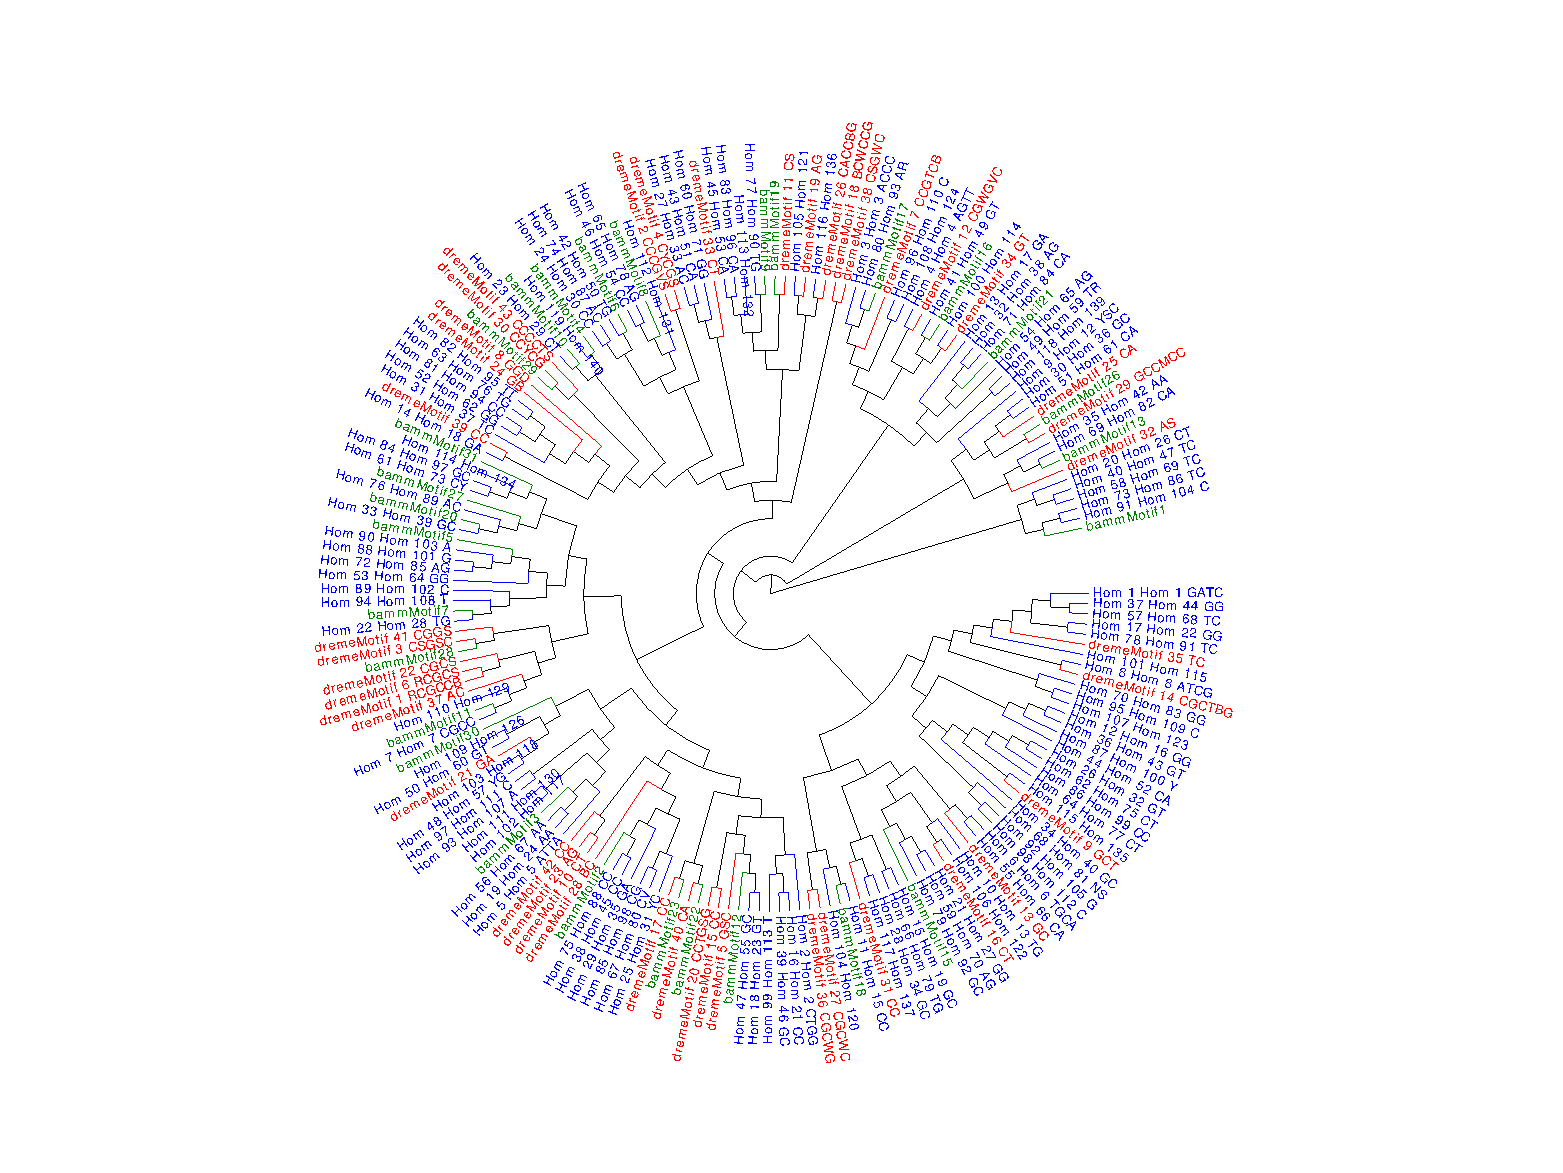
\includegraphics[width= 0.8\textwidth]{stampTree.pdf} 
\caption{{\bf Circular cladogram of Stamp motif alignment.} Detected motifs from HOMER (blue),  DREME (red), and BaMM!motif (green) are clustered due to position weight matrix similarity. }
\label{mainStampTree}
\end{figure}

\begin{figure}[!htbp]
\centering
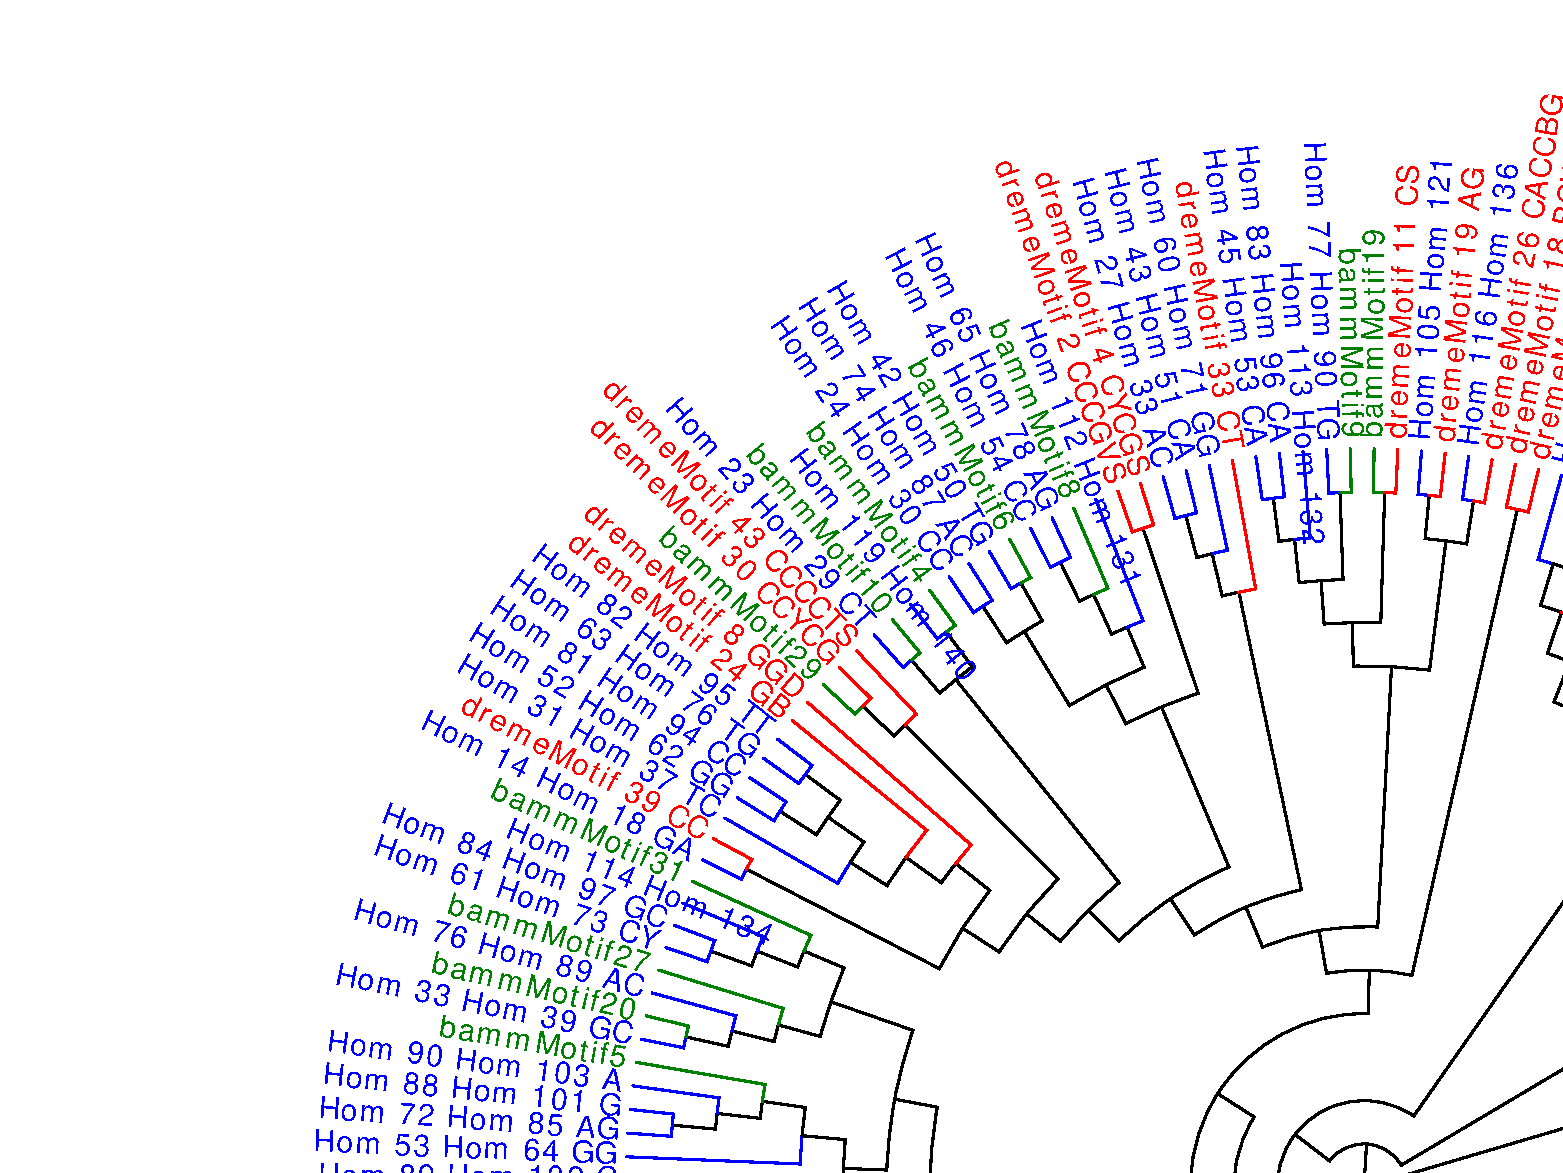
\includegraphics[width= 0.6\textwidth]{stampTreeDetail.pdf} 
\caption{{\bf Zoomed cladogram of Figure \ref{mainStampTree}.} Detected motifs from HOMER (blue),  DREME (red), and BaMM!motif (green) are clustered due to position weight matrix similarity}
\label{treeDetail}
\end{figure}

Using the JASPAR database  \citep{Mathelier2016} as a source for matching detected motifs to TFs, the STAMP algorithm provided five possible TF matches for every motif (Table \ref{5tfs}). 

\begin{table}[!htbp]
\caption{Transcription factor matches for \texttt{Hom\_1\_Hom\_1} motif.}
\label{5tfs}
\centering
\begin{tabular}{ccc}
\toprule[0.2em]
Transcription factor & Stamp match probability & Motif matched \\
\midrule[0.1em]
Snail & $1.28\times10^{-5}$ & GATCACTTGA\\
Nkx2-5 & $1.7\times10^{-3}$ & TCAAGTGATC\\
Mycn & $1.85\times10^{-3}$ & GATCACTTGA\\
Arnt & $1.87\times10^{-3}$ & GATCACTTGA\\
Pax5 & $1.92\times10^{-3}$ & ---------TCAAGTGATC\\
\bottomrule[0.2em]
\end{tabular}
\end{table}

\newpage
Given that $190 \times 5 = 950$ transcription factors were provided, the match probability needed to be adjusted accordingly. Applying a Bonferroni correction to an initial $p < 0.05$ meant that $p$-value $< 5.0\times10^{-5}$ threshold was required. Applying this match threshold, 37 of the 190 motifs were matched to 28 TFs. Of these, eight TFs were matched to motifs from more than one algorithm.
Table \ref{tfsWithMotifs} lists these nine TFs with best match $p$-values.

\begin{table}[!htbp]
\caption{{\bf Transcription factors matched to motifs from at least two algorithms.} Reported are the best Stamp transcription factor match probabilities for HOMER, DREME and BaMM!motif. For the reported transcription factors no motif was found (NMF) by either DREME or BaMM!motif.}
\label{tfsWithMotifs}
\centering
\begin{tabular}{cccc}
\toprule[0.2em]
Transcription factor & HOMER & DREME & BaMM!motif\\
\midrule[0.1em]
IRF1             & $8.15\times10^{-8}$ & NMF & $3.74\times10^{-5}$\\
Snail             & $1.41\times10^{-8}$ & $4.23\times10^{-11}$ & NMF\\
deltaEF1      & $2.94\times10^{-5}$ & $9.60\times10^{-7}$ & NMF\\
Fos              & $2.66\times10^{-6}$ & NMF & $2.46\times10^{-5}$\\
ID1              & $1.50\times10^{-5}$ & NMF & $6.61\times10^{-6}$\\
MEF2A        & $1.95\times10^{-5}$ & NMF & $2.12\times10^{-8}$\\
Prrx2           & $9.64\times10^{-6}$ & NMF & $3.63\times10^{-5}$\\
ESR1         & $4.96\times10^{-5}$ & $3.38\times10^{-5}$ & NMF\\
\bottomrule[0.2em]
\end{tabular}
\end{table}

For each of these transcription factors, more than one motif provided binding sites enriched in the eQTL sequences. Table \ref{totalMotifs} provides the number of matched motifs found for each of the nine TFs.

\begin{table}[!htbp]
\caption{Number of enriched motifs with strong matches to transcription factor}
\label{totalMotifs}
\centering
\begin{tabular}{cc}
\toprule[0.2em]
Transcription factor & Number of motifs\\
\midrule[0.1em]
IRF1             & 7\\
Snail             & 7\\
deltaEF1      & 4\\
Fos           &   4\\
ID1            & 3\\
MEF2A       & 3\\
Prrx2        &  3\\
SQUA       &  3\\
ESR1       &  2\\
\bottomrule[0.2em]
\end{tabular}
\end{table}
\newpage
To more accurately estimate the number of binding sites per sequence per TF, the HOMER annotation software was used as described above (3.1.4 Analysis of the algorithm results). Motifs found by both DREME and BaMM!motif were formatted appropriately to be submitted for annotation by HOMER, as well as the HOMER motifs. The annotation algorithm returns a table of data recording the occurrence of each motif for each of the 10,499 sequences. A simple program was written to add and record the occurrence of all matching motifs for each TF, for each algorithm. This process provides an estimate of the abundance of binding sites for TFs across all sequences. Initially, abundance was measured for all TFs, but the process was then repeated for the nine robust TFs. 

Figure \ref{heatmap} shows the abundance of all motifs over all sequences, and Figure \ref{heatmap2} illustrates the abundance of motifs matching the nine robust TFs over all sequences. As illustrated in Figure \ref{heatmap2}, a relatively large number of motifs that match IRF1 are present in more than half of the 10,499 sequences, but motifs matching Snail, DeltaEF1 and ESR1 are present in moderate to high numbers over all sequences. 


\begin{figure}[!htbp]
\centering
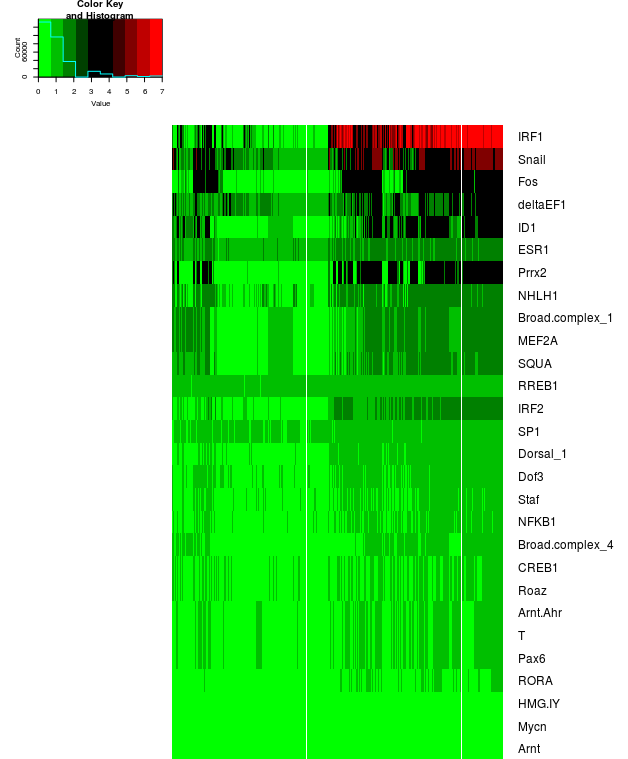
\includegraphics[width= 0.9\textwidth]{heatMapAllTFs.png}
\caption{Abundance of motifs over all eQTL sequences for all transcription factors. Each vertical column indicates the count of motifs for a
particular eQTL sequence that matches the TF in the rows. } 
\label{heatmap}
\end{figure}

\begin{figure}[!htbp]
\centering
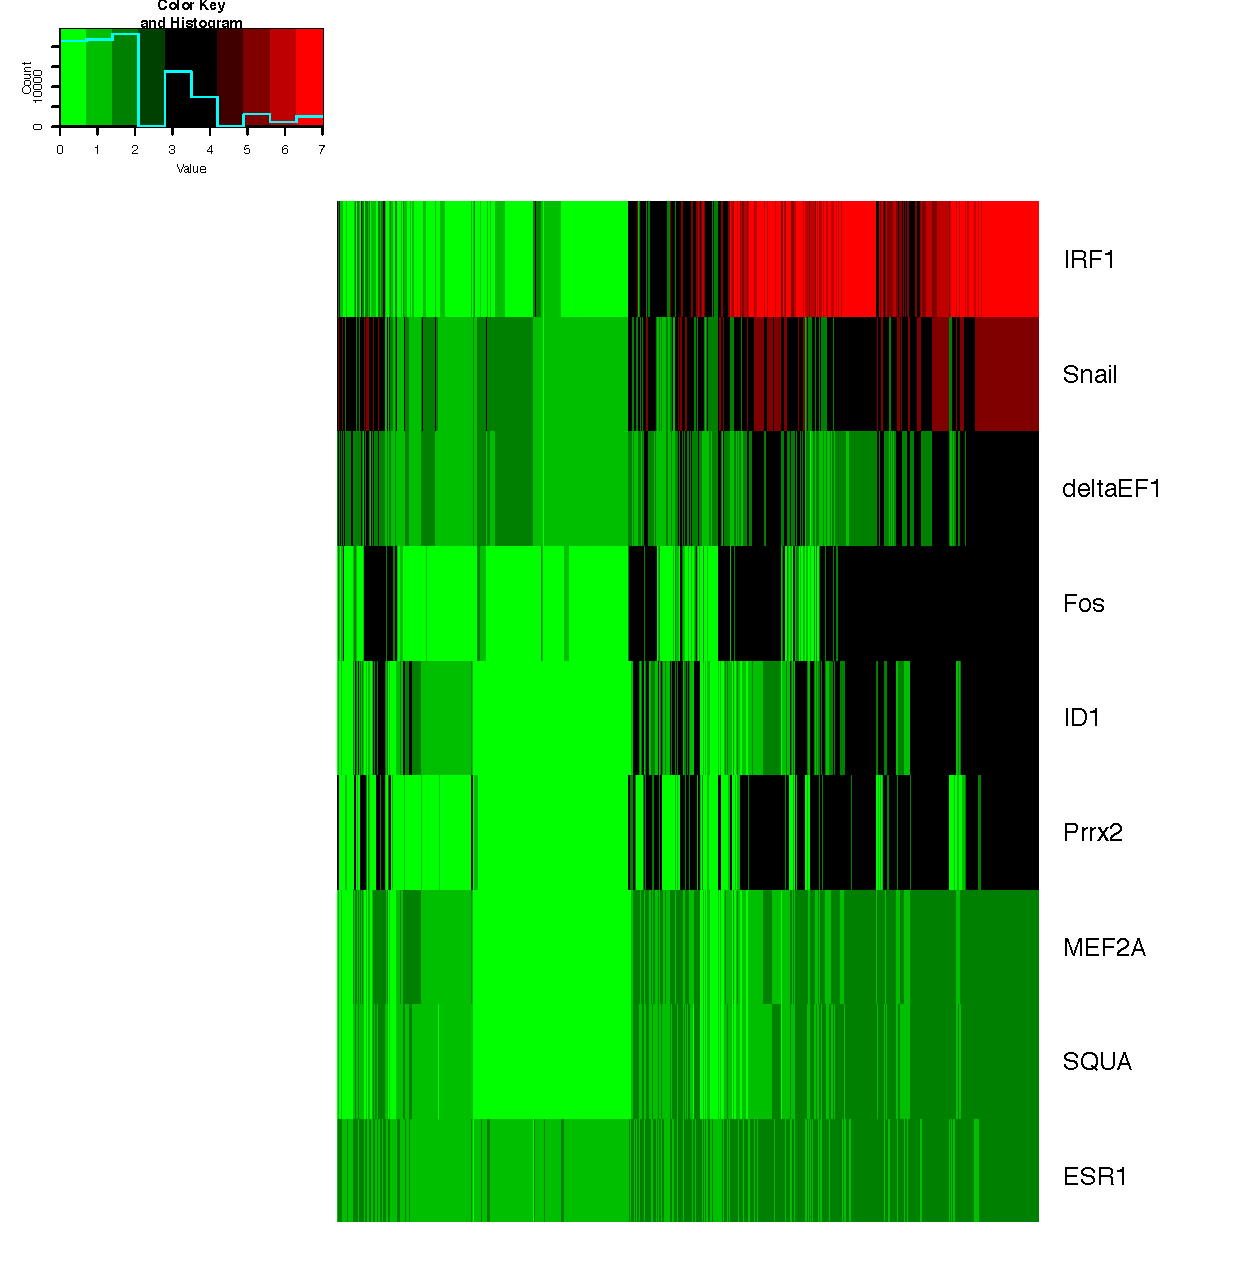
\includegraphics[width= 0.9\textwidth]{HeatmapTopNineTFs.pdf}
\caption{Abundance of motifs over all sequences for 9 transcription factors. Each vertical column indicates the count of motifs for a
particular eQTL sequence that matches the TF in the rows.} 
\label{heatmap2}
\end{figure}

Although these top transcription factors bind to motifs that are enriched in eQTL sequences, they do exist in the null sequences. The process described above, to detect the abundance of TF binding sites across all eQTL sequences, was repeated for the same TF binding sites across the null sequences. A simple summation of binding sites for a TF over all sequences provided the total number of binding sites for each transcription factor for both the eQTL and null sequences (Figure \ref{allMotifComparison}). Table \ref{TFnosEqtl} provides the count of all binding sites for the nine robust TFs in both eQTL and null sequences, and Figure \ref{top9Comparison} provides a graphical illustration of this information.


\begin{figure}[!htbp]
\centering
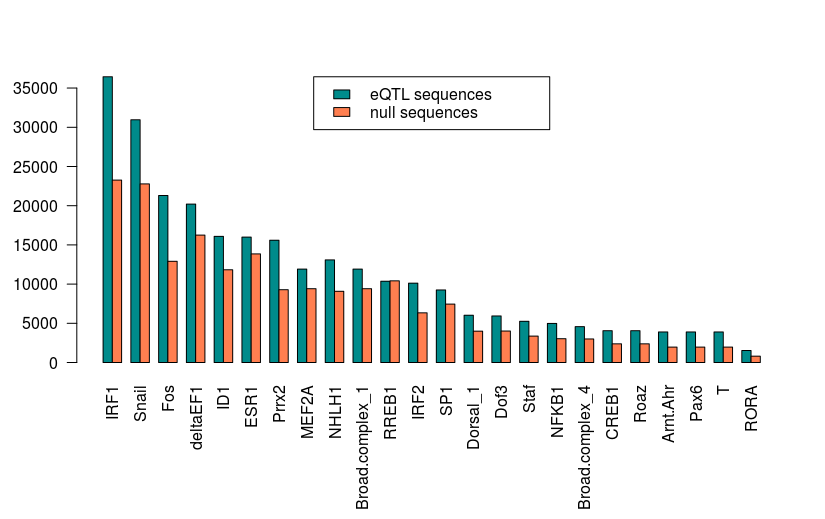
\includegraphics[width= 0.9\textwidth]{AllMotifComparison.png} 
\caption{Comparison of abundance of binding sites for all TFs within eQTL and null sequences. x-axis: All TFs with binding sites enriched in eQTL sequences. y-axis: Abundance of binding sites in eQTL sequences (green) and null sequences (orange)} 
\label{allMotifComparison}
\end{figure}

\begin{table}[!htbp]
\caption{Estimated total number of binding sites for nine TFs enriched in eQTL sequences over both eQTL and null sequences}
\label{TFnosEqtl}
\centering
\begin{tabular}{cccccccccc}
\toprule[0.2em]
& IRF1 & Snail & Fos & deltaEF1 & ID1 & ESR1 & Prrx2 & MEF2A & SQUA\\
\midrule[0.1em]
 eQTL sequences & 36440 & 30954 & 21298 & 20201 & 16087 & 15991 & 15594 & 11914 & 11516\\
 null sequences & 23262 & 22775 & 12908 & 16250 & 11824 & 13851 & 9281 & 9413 & 8825\\
 \bottomrule[0.2em]
\end{tabular}
\end{table}
 

\begin{figure}[!htbp]
\centering
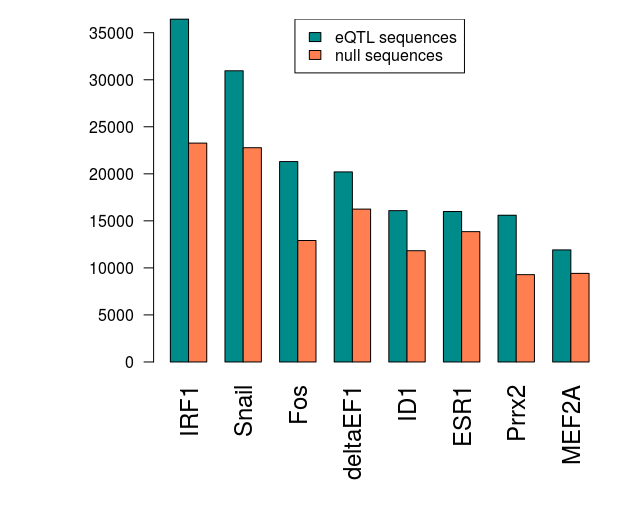
\includegraphics[width= 0.6\textwidth]{Top9TFsComparison.png} 
\caption{Comparison of abundance of binding sites for nine TFs within eQTL and null sequences. x-axis: Nine TFs with binding sites enriched in eQTL sequences. y-axis: Total number of binding sites over all eQTL sequences (green) and null sequences (orange)} 
\label{top9Comparison}
\end{figure}
\newpage

An underlying hypothesis of this project is that eQTL flanking sequences will be rich in biologically active motifs, and, further, that disruption of these motifs through the presence of the eQTL will result in changed regulation of gene or protein expression. Under this hypothesis, if an eQTL is responsible for the disruption of the motif, motifs enriched in the eQTL sequences are more likely to be close to the disruptive variant. A further tool offered by the HOMER software is the distance tool, which calculates average distance from the centre for each motif. This information was used to create graphs of average distance from the variant (both null and eQTL) for all motifs that bind to transcription factors. Figure \ref{distance} illustrates the extent to which binding motifs enriched in eQTL sequences are clustered around either the null variant or the eQTL. The same calculation was performed for motifs enriched in the null sequences. Figure \ref{nullDistance} illustrates the extent to which binding motifs enriched in null sequences are clustered around the null variant or the eQTL. 

\begin{figure}[!htbp]
\centering
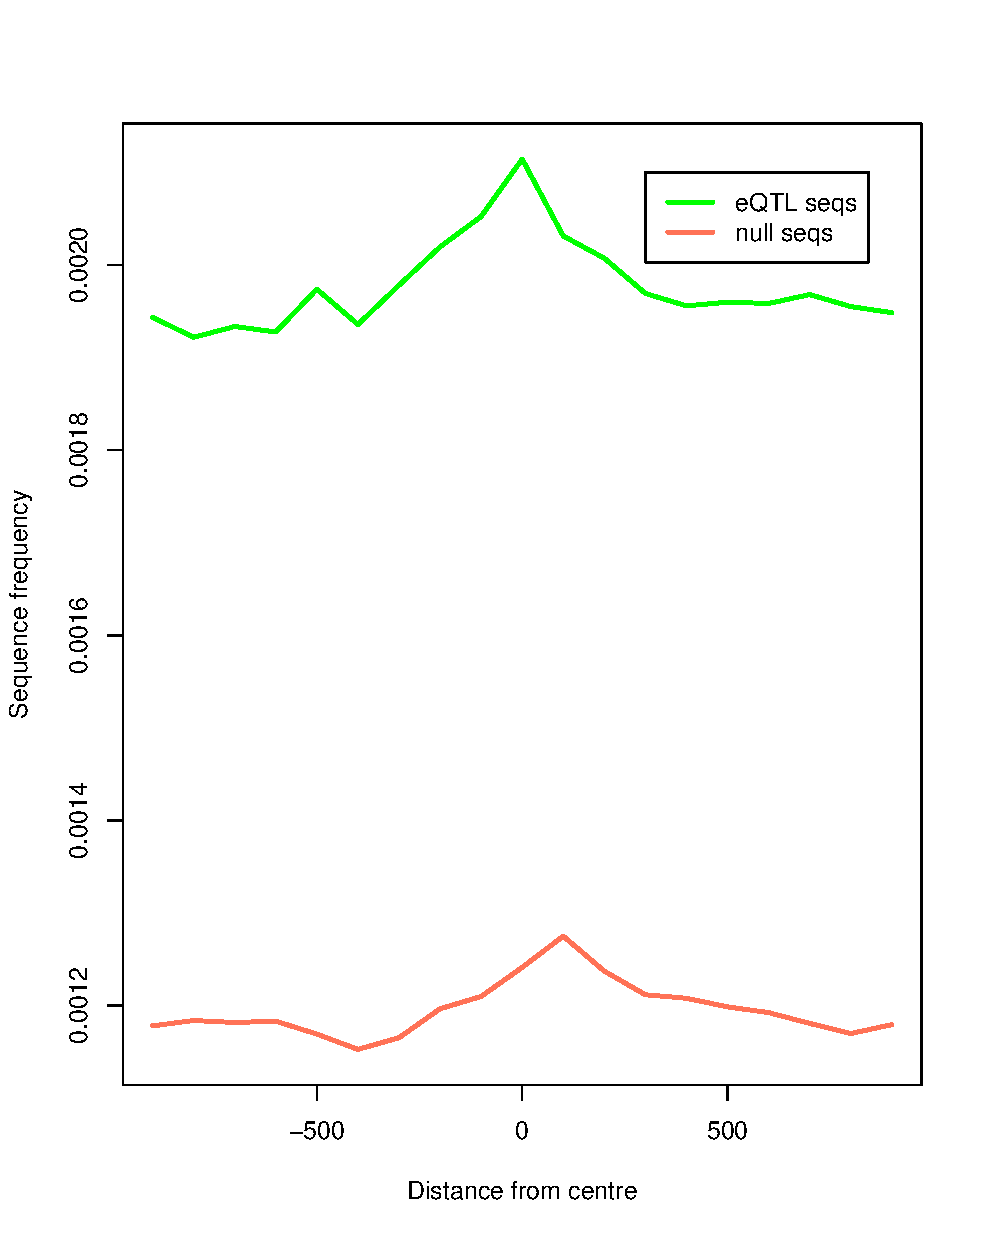
\includegraphics[width= 0.65\textwidth]{RplotEQTLandNullSequencesCompared.pdf} 
\caption{Comparison of distance from eQTL and null variants for TF binding sites enriched in eQTL sequences. x-axis: Distance (in bp) of motif position from the central variant (eQTL or null); y-axis: Frequency of motifs per bp per total sequences}
\label{distance}
\end{figure}

\newpage


\begin{figure}[!ht]
\centering
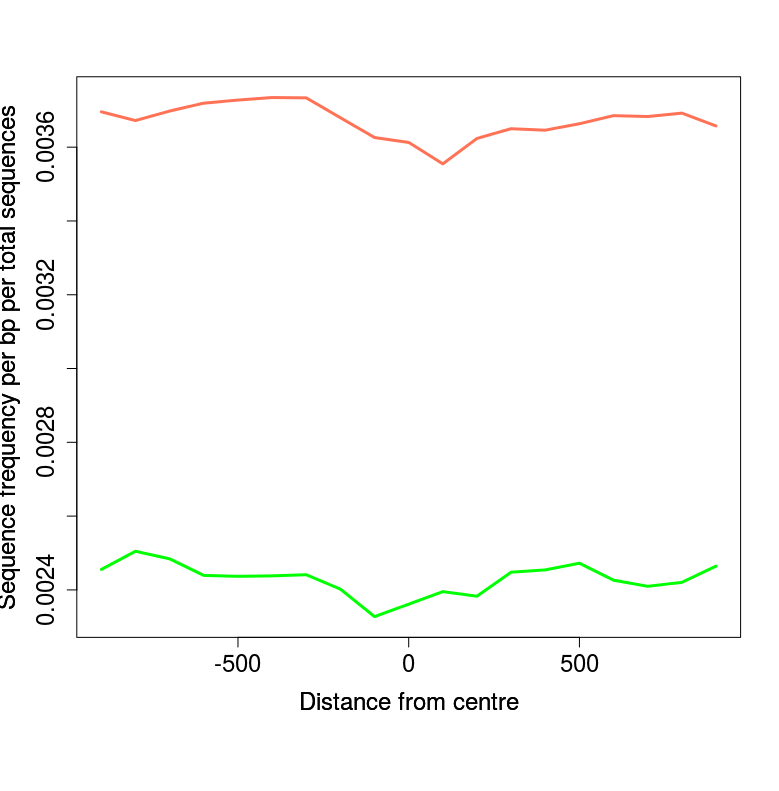
\includegraphics[width= 0.6\textwidth]{RplotNullMotifsCompared.png} 
\caption{Comparison of distance from the centre for TF binding sites enriched in null sequences. x-axis: Distance (in bp) of motif position from the central variant (eQTL or null); y-axis: Frequency of motifs per bp per total sequences}
\label{nullDistance}
\end{figure}

As illustrated in this Figure  \ref{nullDistance}, the sequence frequency of null motifs exceeds the eQTL motif set. As mentioned previously, HOMER found no motifs significantly enriched in the null sequences compared to the eQTL sequences. BaMM!motif found 168 significantly enriched motifs, but these were reduced to six by the AME algorithm. The 39 significantly enriched motifs found by DREME, however, were all accepted as significant by AME. The subsequent analysis by the HOMER annotation tool found a large number of these motifs in both the null and eQTL sequences. The incidence of TFs enriched in null sequences for both eQTL and null sequences is provided for the top eight null enriched TFs in Table \ref{TFnosNull}, and illustrated graphically in Figure \ref{TFnulls}. As illustrated in Table \ref{TFnosNull}, the top four TFs enriched in the null sequences have binding sites more abundant than those of any of the TFs enriched in the eQTL sequences.


\begin{table}[!htbp]
\caption{Total number of binding sites for top eight TFs enriched in null sequences over both eQTL and null sequences}
\label{TFnosNull}
\centering
\begin{tabular}{ccccccccccccc}
\toprule[0.2em]
&Broad-complex{\_}2&Athb-1&ATHB5&MEF2A&TCF1&Hunchback&Prrx2&Evi1\\
\midrule[0.1em]
eQTL Sequences&43805&42640&42105&39450&34040&29375&25668&18827\\
null Sequences&49136&49064&48838&41057&39236&30748&29379&20491\\
 \bottomrule[0.2em]
\end{tabular}
\end{table}

\begin{figure}[!htbp]
\centering
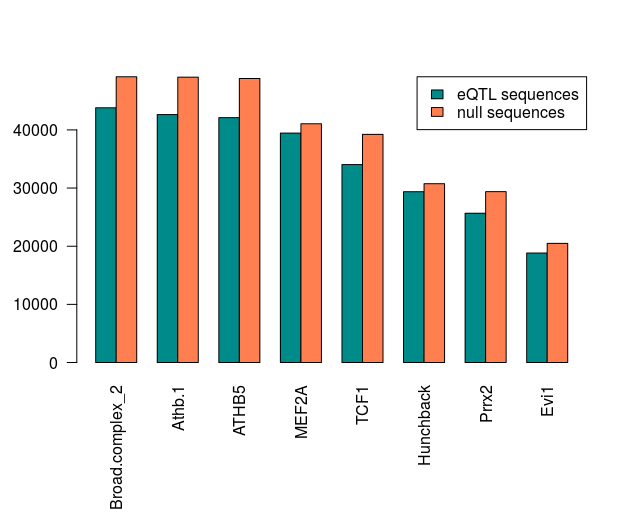
\includegraphics[width= 0.6\textwidth]{RplotNullMotifComparison.png} 
\caption{Comparison of abundance of binding sites for eight null enriched TFs within eQTL and null sequences. x-axis: Eight TFs with binding sites enriched in null sequences. y-axis: Total number of binding sites over all eQTL sequences (green) and null sequences (orange)} 
\label{TFnulls}
\end{figure}

MEF2A and Prrx2 appear as both enriched in eQTL sequences and enriched in null sequences. This apparent anomaly occurs because of the multiple binding sites that have been identified as matching these TFs. The motifs identified as enriched in the eQTL sequences, which match binding sites for MEF2A or Prrx2, are different from those identified as enriched in the null sequences, although these are also matched to alternative binding sites for the same TF. 



Although the focus of this section of the report has been on motifs that were strongly matched to transcription factors, these motifs only represent 19.5\% of the data. No strong matches were found for 80.5\% of motifs. 



\newpage
\section{Discussion}

The correlation of genetic diversity with phenotypic manifestation makes the concept of eQTL mapping very attractive, holding `great promise' as a method to identify causal genetic variants \citep{Pai2015}. However, an understanding of the biological mechanisms by which this diversity regulates gene expression has been challenging \citep{Pai2015, gaffney2013global} . The aim of this project was to identify, quantify, and characterize DNA motifs that are enriched in sequences centred on eQTLs found in whole blood, compared with sequences centred on variants which have no effect on gene expression, in order to highlight differences between eQTLs and null variants that may contribute to these biological mechanisms. This discussion of results will reflect on the findings of this study, before outlining some caveats that limit these findings. The results have also raised more questions and foci for further study, which will form the final part of this section.

\subsection{Discussion of the results}

The first step in motif detection was the identification of reliable algorithms that can provide results that are valid in their discrimination between eQTL and null sequences. Many algorithms exist which can find motifs de novo. Reviews of these motifs have failed to establish any `gold standard' and \citet{tran2014survey} recommend using more than one algorithm to substantiate results. This study found that the HOMER algorithm was reliable and computationally efficient. Although it found many more motifs than either DREME or BaMM!motif, its results were validated by the AME algorithm. It also offers a useful suite of software to annotate motifs. Although BaMM!motif was a promising algorithm, its detection of motifs in sets of null sequences requires further investigation and validation, which motivated further validation of the motifs detected using AME. DREME is part of the well regarded MEME suite, and results indicate that it discriminates between target and background appropriately. DREME also found a substantial number of motifs that were validated by AME, although only four of these were strongly matched to TFs and only two motifs matched TFs that were also bound by motifs found by other algorithms.

The STAMP algorithm proved to be extremely useful in organising data. Its alignment tool provided a useful indication of the validity of different algorithms, in that it illustrated which algorithms found motifs that were similar. A subset of DNA motifs in the region of eQTL are sequence binding sites for transcription factors. The JASPAR database \citep{Mathelier2016} was used by STAMP to match motifs to TFs. This was a convenient tool that allowed identification of TFs strongly matched to the binding sites identified by the motif detection algorithms. 

As part of the validation process, the DREME, HOMER and BaMM!motif algorithms searched for motifs enriched in the sequences flanking null variants compared to the eQTL sequences. It was expected that a small number of unimportant motifs would be found. Although HOMER found no significant results, the overall results contradicted the expectation of small numbers of unimportant motifs, with a total of 46 significant motifs detected by DREME and BaMM!motif, and validated by AME. The STAMP algorithm was used to identify TFs with binding sites matching the motifs. Subsequent analysis found that the number of binding sites for the four most abundant null enriched TFs (Broad-complex{\_}2; Athb-1; ATHB5 and MEF2A), ($>$ 39,000 sites) exceeded the number of binding sites for the most abundant eQTL enriched TF (IRF1 with 36,440 sites).  However, a difference that emerged between these motifs enriched in sequences flanking null variants and motifs enriched in eQTL sequences lies in the distance of these motifs from the variant.
Distance from the variant may be a factor in determining disruption of the binding site. Null-enriched TFs had binding sites that tended to cluster some distance from both the null variant and the eQTL. The converse was true for eQTL-enriched TFs, although binding sites for eQTL-enriched TFs were also more strongly clustered around the eQTL than around the null variant.

Strong matches were found for nine TFs with binding sites found by at least two algorithms. Descriptions of six of these TFs follow \citep{Weizmann2018}:

\paragraph{IRF1 Interferon Regulatory Factor 1:}
The protein encoded by this gene is a transcriptional regulator and tumor suppressor, serving as an activator of genes involved in both innate and acquired immune responses. The encoded protein activates the transcription of genes involved in the body's response to viruses and bacteria, playing a role in cell proliferation, apoptosis, the immune response, and DNA damage response. In particular, IRF1 is a pioneer transcription factor, regulating chromatin accessibility during the differentiation of certain T-cells \citep{Karwacz2017}. As a tumor suppressor, IRF1 both suppresses tumor cell growth and stimulates an immune response against tumor cells. Defects in this gene have been associated with gastric cancer, myelogenous leukemia, and lung cancer \citep{Weizmann2018}.

\paragraph{Snail:}
Involved in induction of the epithelial to mesenchymal transition (EMT), formation and maintenance of embryonic mesoderm, growth arrest, survival and cell migration. Binds to 3 E-boxes of the E-cadherin/CDH1 gene promoter and to the promoters of CLDN7 and KRT8 and, in association with histone demethylase KDM1A which it recruits to the promoters, causes a decrease in dimethylated H3K4 levels and represses transcription. Associates with EGR1 and SP1 to mediate tetradecanoyl phorbol acetate (TPA)-induced up-regulation of CDKN2B, possibly by binding to the CDKN2B promoter region 5-TCACA-3. In addition, may also activate the CDKN2B promoter by itself.


\paragraph{DeltaEF1(also ZEB1)}

Acts as a transcriptional repressor. Inhibits interleukin-2 (IL-2) gene expression. Enhances or represses the promoter activity of the ATP1A1 gene depending on the quantity of cDNA and on the cell type. Represses E-cadherin promoter and induces an epithelial-mesenchymal transition (EMT) by recruiting SMARCA4/BRG1. Represses BCL6 transcription in the presence of the corepressor CTBP1. Positively regulates neuronal differentiation. Represses RCOR1 transcription activation during neurogenesis. Represses transcription by binding to the E box (5-CANNTG-3). Promotes tumorigenicity by repressing stemness-inhibiting microRNAs.

\paragraph{ID1}

ID1 is a member of the helix-loop-helix (HLH) family of transcription factors that are expressed in many tissues. It competitively dimerizes with other members of the HLH family (E2A, E2-2 and HEB), and inhibits their ability to bind DNA and transactivate specific target genes, which are required for cell differentiation In addition to their ability to block differentiation, ID1 genes are expressed in actively proliferating cells, and are known to promote cell proliferation. Thus, deregulation of Id gene expression could contribute to the development of cancer by disrupting these normal cellular processes \citep{Suh2008}. 

\paragraph{Prrx2}

According to \citet{Weizmann2018}, expression is localized to proliferating fetal fibroblasts and the developing dermal layer, with downregulated expression in adult skin. However \citet{juang2016} found that upregulated Prrx2 is associated with poor survival in breast cancer, due to its enhancement of migration, invasion and anchorage?independent growth of MCF10A cells and inducement of partial epithelial mesenchymal transition (EMT).

\paragraph{ESR1}

This gene encodes an estrogen receptor, a ligand-activated transcription factor composed of several domains important for hormone binding, DNA binding, and activation of transcription. The protein localizes to the nucleus where it may form a homodimer or a heterodimer with estrogen receptor 2. Estrogen and its receptors are essential for sexual development and reproductive function, but also play a role in other tissues such as bone. Estrogen receptors are also involved in pathological processes including breast cancer, endometrial cancer, and osteoporosis.


The above TF descriptions are supportive of their presence in whole blood. Two (IRF1 and DeltaEF1) are clearly associated with the immune system. DeltaEF1 can also induce epithelial-mesenchymal transition (EMT), which encourages metastasis. It is generally associated with Snail, which plays a similar role \citep{Bourcy2018}. Snail also associates with SP1 and EGR1 to activate CDKN2A, which plays the opposite role of tumour repression \citep{Hu2010}. SP1 was strongly matched to one binding site enriched in eQTL sequences.

ESR1 is another TF that has been targeted for its role in the spread of cancer. Mutations in the binding domain of ESR1 have been implicated in hormone resistance and anti-estrogen therapies with respect to breast cancer \citep{Griffith2017}

The association of Snail, SP1 and EGR1 is an example of TFs working as a complex rather than as single activators or repressors of genes. Although no binding sites were found for EGR1, \citet{Hu2010} found that the overlapping EGR1/SP1 site (ATCACAGCGGACAGGTATCGGAGCCTAAGGGGG) was the significant motif. A search for this sequence amongst the eQTL flanking regions using FIMO (part of the MEME suite) \citep{Grant2011} found 78,556 motif occurrences with  $p$-value $< 0.001$, maximum $q$-value = 0.515. The $q$-value is an indication of the false discovery rate if the occurrence is accepted as significant, which means that 40,456 of the 78,556 motif occurrences are likely to be false positives. This leaves approximately 38,000 occurrences of the motif over the full set of sequences.

The importance of TF complexes was highlighted by \citet{Jolma2015} and motivated the search for all occurrences of all TFs over all sequences, in order to focus attention on the combinations of TFs in the same sequences. Visualisation of these combinations was accomplished through the heatmaps, which showed a number of combination of TFs that appear to be most abundant in the same sequences. Binding sites for Snail, deltaEF1,  ESR1, RREB1 and SP1 appear in moderate to low numbers over all sequences, but the combination of ID1, MEF2A, Broad-complex{\_}1, SQUA, and, to a lesser extent, IRF1, IRF2, Dorsal{\_}1 and Fos, have the same group of sequences exhibiting no or few binding sites. However, some of these TFs are bound by the same motifs, which provides an alternative explanation for the similarity of their sequence profiles. 

\citet{Jolma2015} also drew attention to alterations in binding specificity of transcription factor pairs, a point already raised through the search for the overlapping SP1/EGR1 site. This may account for some of the unmatched (80\%) of motifs found by the algorithms, which are potentially a set of novel motifs.

It was initially expected that motifs found would form binding sites for known TFs. The large set of unmatched motifs contradicting expectations. These unmatched motifs may indeed be novel sites that bind to TFs, or may represent sites for overlapping or composite binding sites for TF complexes. Other mechanisms, such as splice sites, mRNA sites, or sites that alter the 3-D structure of DNA may also account for many of these sites. 

\subsection{Limitations of the study}
There are a number of caveats on this research which should be taken into account when considering the results:
\begin{enumerate}
\item This analysis has been of eQTLs derived from whole blood gene expression, and the transcription factors identified are likely to be important to the expression of genes in this tissue. However, complex traits result from gene expression in different tissues with possibly different genetic control mechanisms. Whilst these findings are relevant for traits controlled by genes expressed in blood (such as immunity or tumour proliferation), more tissues should be considered to improve our understanding of the complex traits.
\item This analysis also used a single genome reference: Genome Reference Consortium Human Build 37 (GRCh37) \citep{Lander2001}, also known as hg19. Ideally, the same analysis should be performed using different genome references, potentially from different ancestries, to build an understanding of the variation in results depending on the reference genome.
\item The description of the algorithms (either in academic journals or through web pages) are not complete. To a large extent the methods are black boxes, and possible causes of substantial confounding, as well as the convergence properties of the algorithms are left unexplained.
\item In particular, the strong tendency of the BaMM!motif algorithm to provide false positives, as evidenced by the null versus null study, is of substantial concern. In this study other algorithms were used to validate results.
\item The null set does not take into account potentially confounding characteristics such as LD or gene content. 
\item The length of the sequences: the 2001 bp length chosen for sequences was based on the need to avoid overlaps. However, another simple strategy would be to only use eQTLs located on every second chromosome, with null variants located on the alternative chromosomes. This would avoid any possibility of overlap for any length sequence. Longer sequences would increase the likelihood of inclusion of the causal variant, which may be located as far away as 30kb from the known eQTL \citep{wu2018integrative}.
\item The set of motifs that have no match to TFs require further validation.
\item Some of the TFs that formed strong matches to motifs share binding sites. The similarity in sequence abundance profiles may be due to these shared binding sites rather than represent actual combinatory events.
\item The HOMER program that searched for motif occurrence per sequence is a ZOOPS model, returning either zero or one occurrence per sequence. Motif abundance is therefore based on a maximum of one occurrence per sequence, which may be misleading if many instances of the motif occur on a single sequence.
\end{enumerate}

\newpage
\subsection{Directions for future research}
The findings of this study have raised a number of questions that might be considered in future research. 
\begin{enumerate}
\item The concerns raised as limitations need to be addressed. These include:
\begin{enumerate}
\item An extension of the research to include tissues other than whole blood 
\item An extension of the research to include genome references beyond GRCh37 \citep{Lander2001}. 
\item An exploration of the use of high-throughput computing using longer sequences (greater than 30kb) to overcome the eQTL mapping precision problem. 
\item More careful formation of the set of null sequences in order to address possible confounders such as LD or gene content.
\end{enumerate}
\item Four findings of this research provide loci for validation and more in-depth study:
\begin{enumerate}
\item The differential spatial distribution of the motifs about the variant is a promising avenue of study which may distinguish between eQTLs and null variants, but needs to be validated through replication and different study design.

\item The set of transcription factors strongly matched to motifs found by the algorithms might be subjected to more careful analysis to identify known complexes whose binding sites are affected by the eQTL. Shared and/or overlapping binding sites might be identified which may account for some unmatched motifs.

\item Visualisation of TF abundance across all sequences provided evidence of a broad set of sequences that contain zero or very few binding sites for known TFs. These sequences might be isolated for further study of their set of enriched motifs, which, presumably, are located amongst the set of unmatched motifs.

\item The set of unmatched motifs requires further validation through algorithms such as FIMO \citep{Grant2011}. Little has been accomplished with this resource within this study, but this set of potential binding sites may well prove to be a rich source of alternative mechanisms for gene regulation. 
\end{enumerate}
\end{enumerate}

\section{Conclusion}

This project succeeded in its aim of identifying two de novo motif finding algorithms, DREME and HOMER, that can reliably detect and organise motifs enriched in target sequences compared to background sequences. The inclusion of a less robust algorithm, BaMM!motif, was offset by further validation of results through a motif enrichment algorithm, AME. The application of these algorithms resulted in the identification of a number of transcription factors in the vicinity of eQTLs, which may partially explain the mechanism by which these eQTLs affect the regulation of their target genes. The identified TFs include functions affecting the immune system, metastasis and the growth of tumours. Comparison with the same binding sites in sequences associated with null variants indicated that these TFs were less abundant in null sequences and exhibited less tendency to cluster in the proximity of the null variant. 

The findings of this study are limited by the length of the sequences, which may mean that the causal variant may not have been included. Further work should focus on longer sequences, with more attention paid to the configuration of the null set.

Unexpectedly, transcription factor binding sites accounted for a very small percentage of the motifs detected by the algorithms. The set of unmatched motifs identified by the algorithms, after further validation, may provide a rich source of motifs relevant to alternative mechanisms of gene regulation.

\begin{appendices}
\section{Description of algorithms used in the pilot study}
DREME (Discriminative Regular Expression Motif Elicitation) \citep{bailey2011dreme} uses an enumerative algorithm, which is exact in the sense that it examines each possible `word' in the sequence, which is very inefficient, with time increasing exponentially with the size of the motif and the number of sequences. DREME achieves efficiency by limiting the size of the motifs found. Exact enumeration is used for seed motifs restricted to 3-8 base pairs in length, and significance established through comparison with the background sequence, using Fisher's Exact Test. Following this step, the motif is `erased' and the search repeated.
 
HOMER \citep{heinz2010simple} begins by weighting background sequences to resemble the same GC-content distribution of the target sequences, since enrichment scores used in the motif detection algorithms might fail if the distribution of the length of GC content of the target sequences significantly
differs from the background set. Input sequences are then `parsed' to gather all oligos (subsets of 2, 3, and 4 nucleotides long) of the desired motif length and read into an oligo table that records how many times each oligo occurs in the target and background sequences. These frequencies are used to calculate the relative enrichment of each oligo, using the cumulative binomial distribution. The enrichment of longer oligos are calculated using the enrichment values of smaller oligos that make up the longer oligos, similar to the DREME method of combining seed significances. The most enriched oligos are then subjected to a local optimization algorithm which uses a probability matrix to score each oligo according to its similarity to the matrix. By decreasing the detection threshold, more oligos can be included, until an optimal enrichment is found. New probability matrices can then be created at different detection levels, and the matrix that results in the highest enrichment will be used to produce the final motif. This motif is then masked from the sequences and the whole process repeated to find the next motif \citep{homer_ws}.

MotifRG \citep{yao2014discriminative} begins by counting all $k$-mers, for a given motif length $k$, in all sequences. The motifRG algorithm uses logistic regression to fit a model with the best absolute $z$-value (which needs to be above an enrichment threshold). The chosen $k$-mer is used as a seed motif, which is then refined by stepped extension of a given number of nucleotides on each end of the seed at a time. Refinement ends when the $z$-value has not improved after two successive steps. Small perturbations in the seed motif are then tried and accepted if the $z$-value is improved, followed by the extension process. Since a small difference in the $z$-value may not be meaningful, a simple bootstrap test is done if the difference falls below a threshold. A default of 5 random samples of the sequences are used to calculate $z$-values for the new and original motifs. These $z$-values are then subjected to a $t$-test to establish whether their difference is significant.
Once the motif is established, it is masked from all sequences and the process begun again.

STEME (Suffix Tree EM for Motif Elicitation) \citep{reid2011steme} is modelled on the well established MEME algorithm \citep{bailey2009meme}, which uses expectation-maximisation (EM), and this short review begins with a brief description of this process. EM is an extremely robust algorithm but each iteration begins with a time-inefficient initialisation step that generates a matrix of each possible motif and fills in the probability of each base by counting the number of times each base occurs in each position in the set of all motifs and dividing by the number of times it could have occurred (= the number of motifs). The expectation step uses the matrix to calculate the probability of each motif, and then this probability is used to weight the count of bases in the matrix (the maximisation step). The expectation and maximisation (E and M) steps are repeated until convergence is reached and the matrix no longer changes. The EM algorithm is subject to local optimas, and the solution adopted by MEME, to rerun the algorithm with different initial starting positions, results in a running time that is quadratic in the number of sequences and is not practicable with large data sets. STEME modifies the EM algorithm by ignoring all W-mers (subsequences of length W) which have a probability less than some threshold. In addition, STEME uses a suffix tree to iterate over all W-mers. Once the initial matrix is built, it is the content rather than the position of the W-mer that is relevant. A suffix tree can then achieve efficiency over the EM algorithm in two ways: firstly, if any two W-mers are identical they do not have to be repeated; and secondly, partial evaluations are calculated for each step of the suffix tree and shared across W-mers below that node in the tree. In contrast, MEME evaluates every base in each W-mer individually. STEME was still the slowest of these algorithms to run, but its authors claim that it is one order faster than the MEME algorithm with the same data \citep{reid2011steme}.

BaMM!motif (Bayesian Markov model or BaMM) \citep{siebert2016bayesian} addresses the issue that position weight matrices (PWMs) assume independence of each base in the motifs \citep{Jayaram2016}, which may not always be true. By using a Markov model, the BaMM!motif algorithm incorporates the probability of prior nucleotides into the final probability of any nucleotide in a particular position. BaMM!motif begins with a 5th order Markov model and uses expectation maximisation to estimate the transition and emission probabilities of these potential motifs. Probable motifs are lengthened using a Bayesian approach of multiplying the probability of the preceding Markov model with the probability of the proposed additional nucleotide. Because the tables of probabilities produced by this algorithm have incorporated a higher order Markov modelling, the authors refer to them as BaMMs rather than as PWMs, although their layout is the same \citep{siebert2016bayesian}.

DECOD (DECOnvolved Discriminative motif finder) \citep{huggins2011decod} begins with an enumeration step: given a user-specified motif length $k$, all $k$-mers are extracted from the target and background sequences and arranged into a table of frequencies of occurrence. However, after this step, no further analysis is conducted of the actual sequences - all subsequent analysis is of the $k$-mer counts table and PWMs are formed on the basis of frequency of occurrence in target compared to background sequences. This heuristic approach greatly speeds up the algorithm but bears the cost of losing the context of the $k$-mer. This loss of context may mean that overlapping $k$-mers are counted for the same motif more than once, leading to a convolved PWM that is inaccurate. To overcome this problem DECOD adopts a deconvolution process that removes $k$-mers that form a subset of the true motif  \citep{huggins2011decod}.
\end{appendices}

\clearpage

\bibliography{MendeleyLibrary/library}
























\end{document}

